\documentclass[11pt,reqno]{amsart}

\usepackage{amsmath,amssymb,amsthm}
\usepackage[margin=1.1in]{geometry}
\usepackage{microtype}
\usepackage{tikz}
\usepackage[colorlinks=true,linkcolor=blue,citecolor=blue]{hyperref}

\theoremstyle{plain}
\newtheorem{theorem}{Theorem}[section]
\newtheorem{proposition}[theorem]{Proposition}
\newtheorem{lemma}[theorem]{Lemma}
\newtheorem{corollary}[theorem]{Corollary}
\newtheorem{hypothesis}[theorem]{Hypothesis}
\theoremstyle{definition}
\newtheorem{remark}[theorem]{Remark}
\newtheorem{example}[theorem]{Example}
\newtheorem{definition}[theorem]{Definition}
\newtheorem{computation}[theorem]{Computation}

\newcommand{\R}{\mathbb{R}}
\newcommand{\Z}{\mathbb{Z}}
\newcommand{\Q}{\mathbb{Q}}
\newcommand{\C}{\mathbb{C}}
\newcommand{\F}{\mathbb{F}}
\newcommand{\HH}{\mathbb{H}}
\newcommand{\SU}{\mathrm{SU}(2)}
\newcommand{\tr}{\operatorname{tr}}
\newcommand{\Inat}{I^{\natural}}
\newcommand{\HF}{\mathit{HF}}
\newcommand{\CF}{\mathit{CF}}
\newcommand{\Kh}{\mathit{Kh}}
\newcommand{\gr}{\operatorname{gr}}
\newcommand{\rk}{\operatorname{rank}}
\newcommand{\sgn}{\operatorname{sgn}}
\newcommand{\Sig}{\Sigma}
\newcommand{\pill}{\mathcal{P}}
\newcommand{\Rnat}{\mathcal{R}^{\natural}}
\newcommand{\Rp}{\mathcal{R}}
\newcommand{\iss}{\looparrowright}
\newcommand{\bc}{b}
\newcommand{\Qh}[1]{\widehat{Q_{#1}}}

\begin{document}

\title[Instanton homology and Maurer--Cartan deformations]
{The instanton homology of the $(-2,3,q)$ pretzel knots\\
and Maurer--Cartan deformations in the two-arc algebra of the pillowcase}

\author{Bernd J. Wuebben}
\subjclass[2020]{57R58 (primary); 57K10, 57K18, 57K31, 53D40 (secondary)}
\keywords{Singular instanton homology, pretzel knots, pillowcase,
Lagrangian Floer homology, immersed polygons, Atiyah--Floer conjecture,
Khovanov homology}
\date{First version: July 27, 2026. This version: August 15, 2026}

\begin{abstract}
For every odd $q\ge3$ we prove that the reduced singular instanton knot homology of the pretzel knot
$P(-2,3,q)$ is free abelian of rank $q+2$, by squeezing it between Hironaka's Alexander polynomial
and Manion's integral Khovanov homology through the Kronheimer--Mrowka spectral sequence.

On the pillowcase side we work in the wrapped Fukaya subcategory that Cazassus--Herald--Kirk--Kotelskiy
identify with twisted complexes over the two-arc algebra of Kotelskiy--Watson--Zibrowius. There the
higher products vanish, so the Maurer--Cartan equation for a deformation is the finite identity
$(\delta+b)^2=0$, and a filtration lemma proved here reduces the infinite-dimensional morphism
complex between any two finite twisted complexes to three integers. Encoding the $q=7$ curves, we
find that smoothing the Conway-sum curve at any one of four self-intersections yields an exact
Maurer--Cartan element that raises the pairing with the earring from rank $7$ to rank $9=q+2$; the
four objects fall into three homotopy classes, and pairing against a second closure of the same
tangle, whose instanton rank is again computed by the first theorem, isolates one class among all
$82$ single smoothings. That selection is conditional on the conjectural instanton--pillowcase
correspondence and on a stated localization hypothesis. We also show that the formal route through
Gao's representability theorem is closed: the Lagrangian correspondence induced by the $Q_{1/3}$
line is immersed with a triple point, hence not embedded.
\end{abstract}

\maketitle

\section{Introduction}\label{sec:intro}

\subsection{Two homologies for one knot}
Let $K\subset S^3$ be a knot.  On the gauge-theoretic side sits the reduced singular instanton knot
homology $\Inat(K)$ of Kronheimer--Mrowka \cite{KM1,KM2}.  Their integral spectral sequence from
reduced Khovanov homology, their rational identification of $\Inat$ with $KHI$, and the
Alexander-graded Euler characteristic of $KHI$ give
\begin{equation}\label{eq:squeeze}
   \ell(K):=\textstyle\sum_i |a_i(\Delta_K)|
   \;\le\; \dim_{\Q}\Inat(K;\Q)
   \;\le\; \dim_{\Q}\widetilde{Kh}(K;\Q).
\end{equation}
(See \cite[Props.~1.2 and 1.4]{KM2} and \cite[Thm.~1.1]{KMAlex}.)
On the symplectic side sits the pillowcase program of Hedden--Herald--Kirk \cite{HHK1,HHK2}.  Present
$K=(B^3,T_1)\cup_{(S^2,4)}(B^3,T_2)$ as a union of two tangles. The traceless $\SU$ character variety
of the four-punctured sphere is the \emph{pillowcase}
\[
   \pill=(\R/2\pi\Z)^2/\iota,\qquad \iota(\gamma,\theta)=(-\gamma,-\theta),
\]
a two-sphere with four $\Z/2$ orbifold points and symplectic form $d\gamma\wedge d\theta$ on the smooth
locus $\pill^*$ \cite{Lin,HHK1}. Each tangle determines an immersed Lagrangian
$\Rp_{\pi_i}(T_i)\iss\pill^*$ (we write $\iss$ for an immersion) --- the image of its traceless
flat connections under a holonomy
perturbation $\pi_i$.  Their intersections encode traceless representations of the knot group.  The
program seeks a Floer-theoretic counterpart of $\Inat(K)$.

Figure-eight bubbling at self-intersections obstructs the naive composition picture: a strip between
the two Lagrangians can shrink to zero width in a codimension-one degeneration, producing a bubble
whose count deforms the differential and has to be absorbed into a bounding cochain.  Cazassus,
Herald, Kirk and Kotelskiy \cite{CHKK} conjecture that each tangle is assigned an immersed object
equipped with a bounding cochain.  Such an element must satisfy the full Maurer--Cartan equation
\begin{equation}\label{eq:MC}
   \sum_{k\ge0}\mu^k(\bc,\dots,\bc)=0
\end{equation}
and the deformed theory is conjectured to recover $\Inat(K)$ \cite[Conj.~D]{CHKK}.  Equation
\eqref{eq:MC} includes ordered tuples, repeated occurrences of the same generator, and operations of
arbitrarily high order.  Smith proves, conditional on this conjecture, that the cochain assigned to
one Conway-sum tangle in $P(-2,3,5)$ cannot vanish \cite[Thm.~5.9]{Smith}; that argument does not
compute the cochain.

This paper studies both sides for the pretzel family
\begin{equation}\label{eq:family}
   K_q := P(-2,3,q)=\operatorname{num}\big(Q_{-1/2}+Q_{1/3}+Q_{1/q}\big),
   \qquad q\ge3 \text{ odd},
\end{equation}
where $\operatorname{num}$ denotes the numerator closure of the tangle sum and $Q_r$ is the rational
tangle whose traceless character variety is a line of slope $r$, so that the $-2$ band is
$Q_{-1/2}$, following \cite{Smith}. The smallest members
are the torus knots $K_3=T(3,4)=8_{19}$ and $K_5=T(3,5)=10_{124}$ (whose
instanton chain complexes and $\Z/4$ gradings are treated in the companion paper \cite{WuebbenI}),
and the family contains $K_7=P(-2,3,7)$.  We prove an unconditional integral theorem on the
instanton side.  Separately, at $q=7$ we prove an all-orders algebraic statement for the twisted complexes
associated to the specified piecewise-linear curves.  This statement lives in the ungraded
Kotelskiy--Watson--Zibrowius model; it does not identify the resulting deformations with the
bounding-cochain object conjecturally assigned to the tangle.  The lower-order polygon tables for
the other displayed members remain finite experiments.

\subsection{The instanton side: a theorem}
\begin{theorem}\label{thm:inat}
For every odd $q\ge3$,
\[
   \Inat(P(-2,3,q);\Z)\cong\Z^{q+2}.
\]
Consequently its dimensions over $\Q$ and over $\F_2$ are both $q+2$.
\end{theorem}

Hironaka's formula gives an Alexander polynomial with coefficient norm $q+2$, while Manion computes
the reduced integral Khovanov homology as a free abelian group of the same rank.  The rational
Kronheimer--Mrowka bounds therefore agree.  Equality of the rational ranks forces every differential
in their integral spectral sequence to vanish, which gives the stated integral result.  This proof,
given in Section~\ref{sec:inat}, uses no pillowcase model or Atiyah--Floer conjecture.
The smallest members are torus knots whose instanton homology is known, and the case $q=5$ is
Smith's~\cite[\S5]{Smith}; what is new here is the uniform statement for the whole family, and its
integral form.

\subsection{The pillowcase side: an all-orders algebraic result at $q=7$}
Let $\mathcal B$ be the ungraded two-arc algebra used by CHKK and
Kotelskiy--Watson--Zibrowius for the pillowcase with the top-left puncture distinguished
\cite[\S11.5]{CHKK}.  The chart is noncompact, since the distinguished corner is removed, so the category in play is the
\emph{wrapped} Fukaya category, whose morphism complexes are taken after wrapping the ends by a
Hamiltonian.  That is why $\mathcal B$ is infinite dimensional, and why the finiteness of the
morphism homology below has to be proved rather than assumed.  A finite \emph{twisted complex} over
$\mathcal B$ is a finite idempotent module $V$ together with a matrix $\delta$ over $\mathcal B$
satisfying $\delta^2=0$.  Section~\ref{sec:typeD} encodes the $q=7$ piecewise-linear red and blue
curves as twisted complexes $\mathcal E$ (the earring) and $N$ (the Conway sum) over $\mathcal B$.    For a twisted complex $(V,\delta)$ over $\mathcal B$
we write $D_\delta(b)=\delta b+b\delta$ for the endomorphism differential.

\begin{proposition}\label{prop:q7-typeD}
The wrapped morphism homology over $\F_2$ satisfies
\[
 \dim_{\F_2}H\operatorname{Mor}_{\operatorname{Tw}(\mathcal B)}(\mathcal E,N)=7.
\]
At each of four geometric self-intersection orbits of the Conway-sum curve
$\Rp_t(Q_{1/3}+Q_{1/7})$, tabulated in Section~\ref{sec:typeD}, equivariant local
smoothing produces a four-arrow element $b_s\in\operatorname{End}(N)$ such that
\[
 D_N(b_s)=0,\qquad b_s^2=0,
 \qquad
 \dim_{\F_2}H\operatorname{Mor}_{\operatorname{Tw}(\mathcal B)}(\mathcal E,(N,b_s))=9.
\]
\end{proposition}

This proposition is all-orders inside $\operatorname{Tw}(\mathcal B)$: the algebra is associative in
the model used here, so the Maurer--Cartan equation is the finite identity $(\delta_N+b_s)^2=0$.

The proof runs as follows.  Intersections of a curve with the two generating arcs give the
generators, and the segments between them give the arrows, so each piecewise-linear curve becomes an
explicit matrix over $\mathcal B$; after cancelling arrows labelled by idempotents, $N$ has 31
generators and $\mathcal E$ has six.  A local smoothing replaces two arrows of $\delta_N$ by two others, so
$b_s$ has four terms, and $b_s^2=0$ holds for word-length reasons.  The morphism complex over
$\mathcal B$ is infinite dimensional; but it splits by word length into an identity part and a
positive part, the positive part is free over $\F_2[U]$ in each of the three faces, and after unit
cancellation its differential is $U$ times a square-zero constant matrix.  Its homology is therefore
finite, and the whole complex is a mapping cone whose homology has dimension $e+\tau-2r$ in the
notation of Lemma~\ref{lem:wrapped-reduction}.  That is where the dimensions 7 and 9 come from.
Lemma~\ref{lem:wrapped-reduction} applies to any pair of finite twisted complexes over $\mathcal B$,
not only to the two encoded here, and may be of use independently of this calculation.

By Corollary~\ref{cor:q7-classes} the four displayed objects represent exactly three
homotopy-equivalence classes.  One direction is an explicit permutation of generators taking one
smoothed differential to another.  The other uses the homology classes of the underlying curve
components in the torus double cover.  These classes are invariant under regular homotopy, and hence,
by the CHKK immersed-curve classification, under homotopy equivalence.

Propositions~\ref{prop:aux-closure}--\ref{prop:aux-span} and Corollary~\ref{cor:aux-conditional}
then use a second closure to select the common
$S_{18}/S_{25}$ class, conditionally, both from every singleton smoothing that leaves the cancelled module unchanged, at any of the 82
orbits, and from the entire 16-object $\F_2$-span of the four four-arrow elements $b_s$.  The selector
is Theorem~\ref{thm:inat}'s own argument applied a second time: replacing the earring tangle
$\Qh{-1/2}$ by $\Qh{-3/4}$ closes the same Conway sum into a different knot, whose instanton rank is
31 by the same Alexander--Khovanov squeeze, and the three classes pair with the new earring to give
31, 23 and 25.  Requiring both closures to match isolates one class.  Nine of the 82 smoothings change the cancelled
module and are excluded, and duplicate presentations reduce the remaining 73 to 45 distinct elements;
because each is closed and squares to zero, checking the mixed anticommutators of pairs shows that a
whole span of them is Maurer--Cartan.  This does not show that CHKK's
conjectural tangle assignment is represented in that class; that assertion requires a gauge-theoretic
localization or immersed-quilt identification not supplied by the algebraic calculation.

\subsection{A formal route, and why it is blocked}
There is a second, formal way to reach the same object, which would avoid identifying the virtual
chain of every figure-eight bubble: apply a wrapped representability theorem to the Lagrangian
correspondence induced by the $Q_{1/3}$ rational line.  Section~\ref{sec:setup} shows that this route
is unavailable.  Lemma~\ref{lem:surface-reduction} realizes that correspondence as an immersed
Lagrangian surface which is the graph of a symplectic shear away from the seam neighborhoods and has
proper target projection.  Proposition~\ref{prop:partial-triple} then shows it is not embedded: three
distinct transverse points of the partial fiber product share the image
$\bigl((0,\pi/2),(0,\pi/2)\bigr)$.  The mechanism is the denominator.  Along the perturbed reducible
locus over $\gamma=0$ the rational line of slope $1/3$ is cut out by a condition of the form
$3\varphi+4u\in2\pi\Z$, and tripling the angular coordinate wraps the circle three times, so three
branches meet the same fiber; the implicit function theorem then keeps all three, transversally, for
small $t>0$.  Gao's theorem requires an embedded correspondence, so it cannot be
invoked, and Proposition~\ref{prop:yoneda-recognition} records exactly what an immersed replacement
would have to supply.

\subsection{A finite numerical pattern, and what it is not}
Statements labelled \emph{Computation} below are outputs of the finite procedures specified in
Section~\ref{sec:combinatorial}.  They are recorded as data and are not theorems; statements labelled
\emph{Hypothesis} are assumed, not proved.

For the decomposition \eqref{eq:family} take $T_1=\Qh{-1/2}$ and $T_2=Q_{1/3}+Q_{1/q}$.
Section~\ref{sec:setup} builds explicit piecewise-linear curves for the two tangles,
Section~\ref{ss:polygons} defines a finite winding test on them and the rank statistic
\eqref{eq:big-stat} attached to the resulting bigon matrix, and Section~\ref{sec:compute} records the
resulting values.  
First, the statistic takes the values $5,7,15,17$ at $q=5,7,11,13$ against $\dim_{\F_2}\Inat=q+2$, so
the differences are $-2,-2,+2,+2$ and change sign as $\det K_q$ crosses $3$
(Table~\ref{tab:family}).  That is an observation about five displayed rows, one of them imported
from a different tangle presentation~\cite[\S11.6]{HHK2}.  It is not a theorem, and it does not
identify the finite matrix with the differential of any Floer complex.

Second, the search for supports at which low-order polygon terms move that rank by one returns
candidates at $q=5,7,11$, and three of the 55 candidates at $q=11$ fail the square-zero condition
outright (Computation~\ref{comp:cochains}).  The test uses only tabulated monogon, self-bigon and
distinct-crossing self-triangle terms; a geometric double point gives two ordered branch-jump
generators and the search stores only the underlying crossing; and the full series \eqref{eq:MC} is
never tested.  It therefore proves neither existence nor uniqueness of a bounding cochain.

\subsection{Method and scope of claims}
Theorem~\ref{thm:inat} is an unconditional statement about instanton homology.
Proposition~\ref{prop:q7-typeD} is an unconditional statement about two explicitly presented objects
of $\operatorname{Tw}(\mathcal B)$; it neither assumes nor proves the instanton--pillowcase
correspondence.  For the $q=5,11,13$ finite polygon tables, and for an interpretation of the original
$q=7$ polygon table before the type-D encoding, the following four ingredients would be required.
\begin{enumerate}
\item The chosen piecewise-linear resolution must be identified with the actual holonomy-perturbed
character-variety image by more than regular homotopy, or invariance of the relevant curved immersed
object under the allowed regular homotopies must be proved.
\item The winding test must be proved complete and correct for the relevant immersed polygons,
including multiple wrapping, the four orbifold points, and removal of every finite edge-window cutoff.
\item A candidate must be expressed in the ordered branch-jump complex, assigned the required degree,
and shown to satisfy the full Maurer--Cartan equation.  The full deformed series must be defined by a
Novikov filtration or a proved finiteness/nilpotence condition, include repeated inputs at every order,
and square to zero.
\item The resulting immersed object and bounding cochain must be identified with the object assigned
to the tangle by the conjectural instanton--pillowcase correspondence of \cite{CHKK}.
\end{enumerate}
Proposition~\ref{prop:smith-main} identifies the underlying main-component immersion in item (1), up
to regular homotopy, with the cross-paired curve used here.  What remains in that item is a decorated
Floer-invariance statement for the allowed regular homotopy.  The all-orders calculation at $q=7$
removes the finite-window and all-orders issues in items (2) and (3) for every generator-preserving
singleton reconnection at any of the 82 PL self-intersections.  Item (4) remains.  The original closure
rank does not
determine the tangle object; Corollary~\ref{cor:aux-conditional} shows that a second closure
determines its class only after one assumes item (4) and the stated localization hypothesis.
Conditional on that correspondence, Smith's Lemma~5.3 forces the conjectural cochain on the rational
earring tangle to vanish, and Smith's Theorem~5.9 forces a nonzero cochain on the other tangle in the
$q=5$ decomposition \cite{Smith}.  Neither result identifies one of the finite supports computed
here.

\medskip
Section~\ref{sec:inat} proves Theorem~\ref{thm:inat}.  Section~\ref{sec:setup} constructs the
piecewise-linear curves, identifies the blue curve with Smith's main-component model up to regular
homotopy, and records the bigon matrices.  Section~\ref{sec:typeD} proves
Proposition~\ref{prop:q7-typeD} and the statements of \S4.4.  Section~\ref{sec:combinatorial}
defines the finite polygon tables and explains their truncation.  Section~\ref{sec:compute} records
the remaining candidate-support searches and the square-zero check.  Section~\ref{sec:disc}
isolates the geometric and gauge-theoretic identification problem.

\subsection*{Acknowledgements}
The pillowcase model and the geometry reconstructed here are due to Hedden--Herald--Kirk
\cite{HHK1,HHK2}, Cazassus--Herald--Kirk--Kotelskiy \cite{CHKK}, Herald--Kirk \cite{HK}, and Smith
\cite{Smith}; the closed-form Khovanov input is Manion's \cite{Manion}, and the Alexander polynomials
belong to Hironaka's family \cite{Hironaka}.

\section{The instanton rank of the family}\label{sec:inat}

\subsection{The Alexander polynomials}
For $m\ge1$, write $[m]_x=1+x+\cdots+x^{m-1}$.

\begin{proposition}\label{prop:alex}
For every odd $q\ge3$, put
\[
 Q_q(x)=(x-2)[2]_x[3]_x[q]_x+[2]_x[3]_x+[2]_x[q]_x+[3]_x[q]_x.
\]
Then
\begin{equation}\label{eq:alex}
 \Delta_{P(-2,3,q)}(t)\doteq Q_q(-t),
 \qquad
 Q_q(x)=1+x-\sum_{j=3}^{q}x^j+x^{q+2}+x^{q+3},
\end{equation}
where $\doteq$ denotes multiplication by a unit $\pm t^k$.  In particular,
\[
 \ell(P(-2,3,q))=\sum_i|a_i(\Delta)|=q+2.
\]
\end{proposition}

\begin{proof}
Hironaka identifies $P(-2,3,q)$ with the knot denoted $P(2,3,q,-1)$ and proves that its Alexander
polynomial is $Q_{2,3,q}(-t)$, with $Q_{2,3,q}$ equal to the first displayed expression
\cite[Thm.~1.2]{Hironaka}.  Expanding the geometric sums gives the second expression in
\eqref{eq:alex}.  It has four coefficients equal to $1$ and $q-2$ coefficients equal to $-1$.
Substitution $x=-t$ changes signs but not absolute values, so its coefficient norm is
$4+(q-2)=q+2$.
\end{proof}

\begin{remark}
At $q=7$, $Q_7(x)=1+x-x^3-x^4-x^5-x^6-x^7+x^9+x^{10}$ is Lehmer's
polynomial.  The Alexander polynomial is represented by $Q_7(-t)$; substitution $t\mapsto-t$ is part
of Hironaka's formula, not an Alexander-polynomial normalization ambiguity.
\end{remark}

\subsection{The integral spectral sequence}
Manion computes the reduced even Khovanov homology over $\Z$ and proves it is free
\cite[Thm.~1.1]{Manion}.  For $P(-p,r,s)$ with $p$ even, its total rank is
$p^2+(r-p)(s-p)$.  Substituting $(p,r,s)=(2,3,q)$ gives
\begin{equation}\label{eq:kh-rank}
 \widetilde{\Kh}(P(-2,3,q);\Z)\text{ is free of rank }
 4+(3-2)(q-2)=q+2.
\end{equation}
The reduced complex of the mirror is the integral dual complex.  Since the group in
\eqref{eq:kh-rank} is free, the universal coefficient theorem shows that the reduced Khovanov
homology of the mirror is likewise free of rank $q+2$.

\begin{proof}[Proof of Theorem~\ref{thm:inat}]
Kronheimer and Mrowka construct a spectral sequence of abelian groups whose $E_2$ page is the
reduced Khovanov homology of the mirror and whose abutment is $\Inat(K_q;\Z)$
\cite[Prop.~1.2]{KM2}.  After tensoring with $\Q$, \eqref{eq:kh-rank} gives
\[
 \dim_{\Q}\Inat(K_q;\Q)\le q+2.
\]
They also identify $\Inat(K_q;\Q)$ with $KHI(K_q;\Q)$ \cite[Prop.~1.4]{KM2}.  The
Alexander-graded Euler characteristic of $KHI$ is the Alexander polynomial
\cite[Thm.~1.1]{KMAlex}.  Therefore Proposition~\ref{prop:alex} gives
\[
 \dim_{\Q}\Inat(K_q;\Q)=\dim_{\Q}KHI(K_q;\Q)
 \ge \ell(K_q)=q+2.
\]
Thus both rational bounds are equal.  Total dimension cannot increase from one page to the next in
a spectral sequence of finite-dimensional vector spaces, so equality of the $E_2$ and $E_\infty$
dimensions forces every differential after tensoring with $\Q$ to vanish.

It remains to use the integral spectral sequence.  Its $E_2$ page is free of rank $q+2$ by the
preceding mirror-duality argument.  Inductively each page is free, and a homomorphism between free
abelian groups whose rationalization is zero is itself zero.
Hence every integral differential vanishes.  The associated graded group of $\Inat(K_q;\Z)$ is
free of rank $q+2$; its finite filtration splits because extensions of free abelian groups split.
This proves $\Inat(K_q;\Z)\cong\Z^{q+2}$.  The assertions over $\Q$ and $\F_2$ follow by base change
and the universal coefficient theorem.
\end{proof}

\begin{remark}
The rational squeeze is the argument Smith uses for $P(-2,3,5)$ \cite[proof of Thm.~5.9]{Smith}.
The freeness in Theorem~\ref{thm:inat} additionally uses Manion's integral calculation and collapse of
the integral spectral sequence.  We also note
$\det P(-2,3,q)=|{-6}+3q-2q|=|q-6|$, which never vanishes and equals $1$ exactly for $q=5,7$: precisely
the members whose double branched cover is an integral homology sphere.
\end{remark}

\section{Piecewise-linear curve models for the family}\label{sec:setup}

\subsection{The pillowcase and the two model curves}
We use $\SU$ as the unit quaternions; a traceless element is a purely imaginary unit. The traceless
character variety of the four-punctured sphere is the pillowcase of the introduction, with coordinates
$(\gamma,\theta)$, involution $\iota(\gamma,\theta)=(-\gamma,-\theta)$, and corners
$\{0,\pi\}^2$ \cite{Lin,HHK1}. We work on the double cover $T^2$, where curves lift to
$\iota$-invariant families; the finite bookkeeping is described in
Section~\ref{sec:combinatorial}. A rational tangle $Q_r$ has for its character variety a straight
line of slope $r$ through the corners \cite{HHK1}.  The following operations are used to build the
piecewise-linear models.  Proposition~\ref{prop:smith-main} identifies the underlying blue
main-component immersion; it does not identify its Floer decoration:
\begin{itemize}
\item \emph{Conway sum.} On the pillowcase, $T_1+T_2$ is the fiber product over $\gamma$: the
$\theta$-coordinates add, and over each seam $\gamma\in\{0,\pi\}$ a circle of reducibles appears when
both summands are non-abelian there \cite[Thms.~3.15 and 3.26]{Smith}. Perturbing resolves each circle by a
diagonal cut-and-paste \cite[Thm.~4.22]{Smith}, adding one self-intersection per circle.
\item \emph{Earring.} $\Qh{r}$ replaces the arc of $Q_r$ by the Herald--Kirk figure-eight: the doubled
arc closing through the corner folds, with one pinch \cite[Def.~6.7]{HK}.  This specifies the finite
curve used below; it does not specify a bounding cochain.
\end{itemize}
Write $L_{q,\mathrm{PL}}$ for the blue curve obtained from the rational lines of slopes $1/3$ and
$1/q$ by the displayed fiber product and the crossed local pairing at every seam-fiber circle.
Following \cite{Smith} we call the two circles $\gamma\in\{0,\pi\}$ the \emph{seams} of the
pillowcase; they are unrelated to the seams of a quilt.
For the decomposition \eqref{eq:family} the $-2$ band is constant, so
\textbf{red} $=\Rnat(\Qh{-1/2})$ is \emph{independent of $q$} (one immersed circle, one pinch), while
\textbf{blue} $=\Rp_t(Q_{1/3}+Q_{1/q})$ varies: two seams, $q-1$ resolved fiber circles, and a single
proper immersed arc whose self-intersection count grows with $q$ (40 at $q=5$, 82 at $q=7$,
225 at $q=11$). We require $\gcd(q,3)=1$ (else corner circles appear); this excludes
$q=3,9,15,\dots$ from the members we compute, but not from Theorem~\ref{thm:inat}.  (The $q=3$
external value is Hedden--Herald--Kirk's, from their own presentation; see \S\ref{ss:gate}.)

\begin{proposition}[Identification of the main immersion]\label{prop:smith-main}
Let $q$ be odd and $\gcd(q,3)=1$.  For all sufficiently small positive values of Smith's
$C_3$-perturbation parameter, the image in the pillowcase of the main component of
$\Rp_t(Q_{1/3}+Q_{1/q})$ is regularly homotopic to $L_{q,\mathrm{PL}}$.

Any auxiliary circle components can be excluded from a fixed Floer pairing by an arbitrarily small
perturbation of the complementary tangle.  This auxiliary-component statement remains valid when
either tangle carries an earring.
\end{proposition}

\begin{proof}
Smith's rational-tangle calculation identifies the two character varieties with straight intervals
of slopes $1/3$ and $1/q$ \cite[Prop.~2.27]{Smith}.  Rational tangles of finite slope form a good pair
without preliminary perturbations \cite[example following Thm.~3.26]{Smith}.  Because their
denominators $3$ and $q$ are coprime, the sum has no corner circles
\cite[discussion following Prop.~5.8]{Smith}; hence every seam-fiber circle is internal.

Smith's cross-resolution theorem replaces a neighborhood of each internal circle by two intervals
joining opposite abelian ends \cite[Thm.~4.22]{Smith}.  This is exactly the crossed local pairing in
the definition of $L_{q,\mathrm{PL}}$.  The theorem's regular-homotopy conclusion, together with its
rotated-perturbation version \cite[Prop.~4.23]{Smith}, therefore gives the first assertion.  Finally,
Smith's auxiliary-component avoidance result permits an arbitrarily small perturbation of any fixed
complementary one-manifold so that its image misses every auxiliary circle, and explicitly includes
the earring case \cite[Prop.~5.7]{Smith}.
\end{proof}

\subsection{The $Q_{1/3}$ correspondence is immersed but not embedded}
Write $P_1,P_2,P_3$ for the pillowcases of the three boundary spheres of Smith's $C_3$
configuration, $P^-$ for a pillowcase with the sign of its symplectic form reversed, $P^*$ for the
smooth locus, and $C_3\subset P_1^-\times P_2^-\times P_3$ for his three-sphere correspondence; the
superscript $\mathrm{reg}$ denotes its regular Lagrangian locus \cite[Cor.~4.11]{Smith}.

\begin{lemma}[Reduction to a correspondence between surfaces]
\label{lem:surface-reduction}
Let $A_{1/3}\iss P_1$ be the rational line for $Q_{1/3}$, and let
$C_{3,t}^{\mathrm{reg}}\iss P_1^-\times P_2^-\times P_3$ denote the regular Lagrangian locus of
Smith's perturbed $C_3$ correspondence.  Wherever the fiber product is transverse, set
\[
 F_{1/3,t}:=A_{1/3}\times_{P_1}C_{3,t}^{\mathrm{reg}}
       \iss P_2^-\times P_3.
\]
Then $F_{1/3,t}$ is an immersed Lagrangian surface.  On a torus-cover chart of the unperturbed main
stratum with $\gamma\notin\{0,\pi\}$, a branch of $A_{1/3}$ has
$\theta_1=\gamma/3+c$, and $F_{1/3,0}$ is the graph of the symplectic shear
\[
 (\gamma,\eta)\longmapsto
 (\gamma,\eta+\gamma/3+c).
\]
On every compact subset of such a chart, the projection of $F_{1/3,t}$ to $P_2$ remains a local
diffeomorphism for all sufficiently small $t>0$.  After composition with the rational line for
$Q_{1/7}$, the complement of these graph charts is contained in neighborhoods of the six internal
fiber circles used in Proposition~\ref{prop:smith-main}.  If the fiber product is transverse along
the entire regular locus, then the target projection $F_{1/3,t}\to P_3^*$ is proper.
\end{lemma}

\begin{proof}
On the unperturbed main stratum, Smith's boundary-coordinate formulas give
\[
 p_1=(\gamma,\beta),\qquad
 p_2=(\gamma,\theta-\beta),\qquad
 p_3=(\gamma,\theta).
\]
Imposing $\beta=\gamma/3+c$ and writing $\eta=\theta-\beta$ gives the displayed graph.  Its pullback
preserves $d\gamma\wedge d\theta$, since
$d\gamma\wedge d(\eta+\gamma/3+c)=d\gamma\wedge d\eta$.  The standard transverse-composition
lemma therefore makes the fiber product Lagrangian.  The projection to $P_2$ is a local
diffeomorphism at $t=0$ away from the seams; this property persists on compact subsets by the
implicit-function theorem.  For $Q_{1/3}$ and $Q_{1/7}$, Smith's rational-line and coprime-denominator
analysis leaves six internal fiber circles, and \cite[Theorem~4.22]{Smith} replaces precisely their neighborhoods
by the crossed pieces used to construct $L_{7,\mathrm{PL}}$.

For properness, let $\overline A_{1/3}$ be the compact rational arc in the full pillowcase and set
\[
 \overline F_{1/3,t}:=
 \overline A_{1/3}\times_{P_1}\mathcal R_{D_t}(C_3).
\]
This is a closed subset of a compact space.  Smith proves that the boundary restriction of
$\mathcal R_{D_t}(C_3)$ lies in
$P_1^*\times P_2^*\times P_3^*$ or in the product of the three corner strata, with no mixed
strata \cite[Prop.~4.3]{Smith}; its regular Lagrangian locus is the former
\cite[Cor.~4.11]{Smith}.  Hence every point of
$\overline F_{1/3,t}\setminus F_{1/3,t}$ maps to a corner of $P_3$.  If $K\subset P_3^*$ is compact,
its inverse image is therefore the compact set
$\overline p_3^{-1}(K)\subset\overline F_{1/3,t}$ and is contained in $F_{1/3,t}$.  This is the
definition of properness.
\end{proof}

\begin{proposition}[A triple-point obstruction]\label{prop:partial-triple}
For every sufficiently small $t>0$, the partial fiber product in
Lemma~\ref{lem:surface-reduction} has three distinct transverse points whose images in
$P_2^*\times P_3^*$ are all
\[
 \bigl((0,\pi/2),(0,\pi/2)\bigr).
\]
Consequently, $F_{1/3,t}\to P_2^-\times P_3$ is not embedded.
\end{proposition}

\begin{proof}
Work in the unit quaternions and put
\[
 v(\varphi)=\cos\varphi\,\mathbf i+\sin\varphi\,\mathbf k.
\]
Fix $\gamma=0$ and $\theta=\pi/2$ in Smith's parametrization, so that
$a=b=\mathbf i$ and $c=d=\mathbf j$.  For $\beta=0$ or $\pi$, write
\[
 (\varphi,u)=
 \begin{cases}
  (\pi/2-\alpha,\ t\sin\alpha),&\beta=0,\\
  (\pi/2+\alpha,-t\sin\alpha),&\beta=\pi.
 \end{cases}
\]
Then $x=v(\varphi)$ and the perturbation element is $p=e^{-u\mathbf j}$.  Direct quaternion
multiplication shows that $y=xp^{-1}a^{-1}pb$ is purely imaginary.  Thus Smith's defining equation
$\operatorname{Re}(y)=0$ holds identically along these two one-parameter families.

On the torus cover, the first boundary value has coordinates
\[
 (\gamma_1,\theta_1)=(2u,\varphi+2u).
\]
The equation for the rational line $A_{1/3}$ is therefore
$3\varphi+4u\in2\pi\Z$.  It gives the following three equations near the indicated roots:
\begin{align*}
 3(\pi/2-\alpha)+4t\sin\alpha&=0,
     &\alpha&\longrightarrow\pi/2,\quad \beta=0,\\
 3(\pi/2+\alpha)-4t\sin\alpha&=2\pi,
     &\alpha&\longrightarrow\pi/6,\quad \beta=\pi,\\
 3(\pi/2+\alpha)-4t\sin\alpha&=4\pi,
     &\alpha&\longrightarrow5\pi/6,\quad \beta=\pi.
\end{align*}
At $t=0$ the three derivatives with respect to $\alpha$ are $-3,3,3$.  The implicit-function
theorem consequently gives three solutions for all sufficiently small $t>0$.  They are distinct
because their limiting $x$-values are distinct.  Moreover, their first-boundary $\gamma$-coordinate
has absolute value $2t\sin\alpha>0$, so none lies over a corner of $P_1$.

The second-boundary words simplify, using $xp=p^{-1}x$, to
\[
 (a_2,b_2,c_2,d_2)
 =\bigl(v(\varphi+2u),v(\varphi+2u),\mathbf j,\mathbf j\bigr).
\]
Hence $p_2=(0,\pi/2)$ at all three points, while
$(a,b,c,d)=(\mathbf i,\mathbf i,\mathbf j,\mathbf j)$ gives
$p_3=(0,\pi/2)$.  Finally, differentiation of the two local defining equations gives
$\partial_\beta\operatorname{Re}(y)=-2t\sin^2\alpha+O(t^2)$ and
$\partial_\alpha(3\theta_1-\gamma_1)=\pm3+O(t)$.  Thus the fiber product is transverse at all
three points for small $t>0$.
\end{proof}

\begin{figure}[ht]
\centering
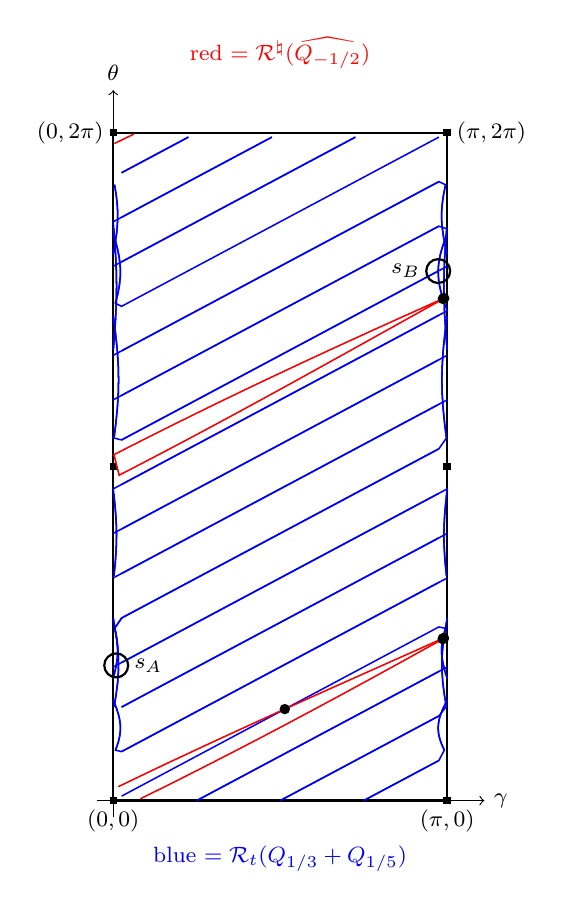
\begin{tikzpicture}[scale=1.35]
% --- Figure 1 curves, generated by pillowcase/make_figure.py (inlined) ---
% AUTO-GENERATED by pillowcase/make_figure.py -- the q=5 PL model curves.
%% blue folded into 52 pieces; red (both lifts) into 10 pieces.
\draw[thick] (0,0) rectangle (3.14159,6.28319);
\foreach \y in {0,3.14159,6.28319}{\fill (-0.035,\y-0.035) rectangle (0.035,\y+0.035); \fill (3.14159-0.035,\y-0.035) rectangle (3.14159+0.035,\y+0.035);}
\node[below] at (0,0) {\footnotesize $(0,0)$};
\node[below] at (3.1416,0) {\footnotesize $(\pi,0)$};
\node[left] at (0,6.2832) {\footnotesize $(0,2\pi)$};
\node[right] at (3.1416,6.2832) {\footnotesize $(\pi,2\pi)$};
\draw[->] (-0.15,0)--(3.4916,0) node[right] {\footnotesize $\gamma$};
\draw[->] (0,-0.15)--(0,6.6832) node[above] {\footnotesize $\theta$};
\draw[blue,line width=0.55pt] (0.0000,5.4454) -- (0.1571,5.5292) -- (0.3142,5.6130) -- (0.4712,5.6968) -- (0.6283,5.7805) -- (0.7854,5.8643) -- (0.9425,5.9481) -- (1.0996,6.0319) -- (1.2566,6.1156) -- (1.4137,6.1994) -- (1.4923,6.2413);
\draw[blue,line width=0.55pt] (1.5708,0.0000) -- (1.7279,0.0838) -- (1.8850,0.1676) -- (2.0420,0.2513) -- (2.1991,0.3351) -- (2.3562,0.4189) -- (2.5133,0.5027) -- (2.6704,0.5864) -- (2.8274,0.6702) -- (2.9845,0.7540) -- (3.0631,0.7959);
\draw[blue,line width=0.55pt] (3.1336,0.8836) -- (3.1150,0.9948) -- (3.1000,1.1126) -- (3.0923,1.2305) -- (3.0926,1.3352) -- (3.0974,1.4137) -- (3.1056,1.4923) -- (3.1186,1.5839) -- (3.1411,1.7148);
\draw[blue,line width=0.55pt] (3.1402,4.5553) -- (3.1221,4.4113) -- (3.1092,4.2935) -- (3.1012,4.2019) -- (3.0937,4.0710) -- (3.0916,3.9532) -- (3.0947,3.8223) -- (3.1030,3.6914) -- (3.1173,3.5474) -- (3.1341,3.4099) -- (3.0631,3.3091) -- (2.9060,3.2254) -- (2.7489,3.1416) -- (2.5918,3.0578) -- (2.4347,2.9740) -- (2.2777,2.8903) -- (2.1206,2.8065) -- (1.9635,2.7227) -- (1.8064,2.6389) -- (1.6493,2.5552) -- (1.4923,2.4714) -- (1.3352,2.3876) -- (1.1781,2.3038) -- (1.0210,2.2201) -- (0.8639,2.1363) -- (0.7069,2.0525) -- (0.5498,1.9687) -- (0.3927,1.8850) -- (0.2356,1.8012) -- (0.0785,1.7174) -- (0.0135,1.6205) -- (0.0299,1.5420) -- (0.0392,1.4713) -- (0.0418,1.4085) -- (0.0394,1.3535) -- (0.0339,1.3064) -- (0.0258,1.2593) -- (0.0004,1.1493);
\draw[blue,line width=0.55pt] (0.0011,5.1417) -- (0.0163,5.2281) -- (0.0338,5.3538) -- (0.0411,5.4559) -- (0.0412,5.5423) -- (0.0363,5.6208) -- (0.0273,5.6994) -- (0.0126,5.7936);
\draw[blue,line width=0.55pt] (0.0785,5.9062) -- (0.2356,5.9900) -- (0.3927,6.0737) -- (0.5498,6.1575) -- (0.7069,6.2413);
\draw[blue,line width=0.55pt] (0.7854,0.0000) -- (0.9425,0.0838) -- (1.0996,0.1676) -- (1.2566,0.2513) -- (1.4137,0.3351) -- (1.5708,0.4189) -- (1.7279,0.5027) -- (1.8850,0.5864) -- (2.0420,0.6702) -- (2.1991,0.7540) -- (2.3562,0.8378) -- (2.5133,0.9215) -- (2.6704,1.0053) -- (2.8274,1.0891) -- (2.9845,1.1729) -- (3.0631,1.2147);
\draw[blue,line width=0.55pt] (3.1416,5.0265) -- (2.9845,4.9428) -- (2.8274,4.8590) -- (2.6704,4.7752) -- (2.5133,4.6914) -- (2.3562,4.6077) -- (2.1991,4.5239) -- (2.0420,4.4401) -- (1.8850,4.3563) -- (1.7279,4.2726) -- (1.5708,4.1888) -- (1.4137,4.1050) -- (1.2566,4.0212) -- (1.0996,3.9375) -- (0.9425,3.8537) -- (0.7854,3.7699) -- (0.6283,3.6861) -- (0.4712,3.6024) -- (0.3142,3.5186) -- (0.1571,3.4348) -- (0.0785,3.3929);
\draw[blue,line width=0.55pt] (0.0075,3.4099) -- (0.0243,3.5474) -- (0.0385,3.6914) -- (0.0469,3.8223) -- (0.0500,3.9532) -- (0.0479,4.0710) -- (0.0404,4.2019) -- (0.0324,4.2935) -- (0.0194,4.4113) -- (0.0014,4.5553);
\draw[blue,line width=0.55pt] (0.0005,1.7148) -- (0.0229,1.5839) -- (0.0360,1.4923) -- (0.0442,1.4137) -- (0.0489,1.3352) -- (0.0493,1.2305) -- (0.0416,1.1126) -- (0.0266,0.9948) -- (0.0080,0.8836);
\draw[blue,line width=0.55pt] (0.0785,0.8796) -- (0.2356,0.9634) -- (0.3927,1.0472) -- (0.5498,1.1310) -- (0.7069,1.2147) -- (0.8639,1.2985) -- (1.0210,1.3823) -- (1.1781,1.4661) -- (1.3352,1.5499) -- (1.4923,1.6336) -- (1.6493,1.7174) -- (1.8064,1.8012) -- (1.9635,1.8850) -- (2.1206,1.9687) -- (2.2777,2.0525) -- (2.4347,2.1363) -- (2.5918,2.2201) -- (2.7489,2.3038) -- (2.9060,2.3876) -- (3.0631,2.4714);
\draw[blue,line width=0.55pt] (3.1416,3.7699) -- (2.9845,3.6861) -- (2.8274,3.6024) -- (2.6704,3.5186) -- (2.5133,3.4348) -- (2.3562,3.3510) -- (2.1991,3.2673) -- (2.0420,3.1835) -- (1.8850,3.0997) -- (1.7279,3.0159) -- (1.5708,2.9322) -- (1.4137,2.8484) -- (1.2566,2.7646) -- (1.0996,2.6808) -- (0.9425,2.5970) -- (0.7854,2.5133) -- (0.6283,2.4295) -- (0.4712,2.3457) -- (0.3142,2.2619) -- (0.1571,2.1782) -- (0.0785,2.1363);
\draw[blue,line width=0.55pt] (0.0000,4.1888) -- (0.1571,4.2726) -- (0.3142,4.3563) -- (0.4712,4.4401) -- (0.6283,4.5239) -- (0.7854,4.6077) -- (0.9425,4.6914) -- (1.0996,4.7752) -- (1.2566,4.8590) -- (1.4137,4.9428) -- (1.5708,5.0265) -- (1.7279,5.1103) -- (1.8850,5.1941) -- (2.0420,5.2779) -- (2.1991,5.3617) -- (2.3562,5.4454) -- (2.5133,5.5292) -- (2.6704,5.6130) -- (2.8274,5.6968) -- (2.9845,5.7805) -- (3.0631,5.8224);
\draw[blue,line width=0.55pt] (3.1258,5.7936) -- (3.1072,5.6994) -- (3.0959,5.6208) -- (3.0898,5.5423) -- (3.0898,5.4559) -- (3.0936,5.4009) -- (3.1075,5.2988) -- (3.1211,5.2281) -- (3.1402,5.1417);
\draw[blue,line width=0.55pt] (3.1411,1.1493) -- (3.1174,1.2278) -- (3.1036,1.2828) -- (3.0950,1.3299) -- (3.0900,1.3771) -- (3.0896,1.4399) -- (3.0941,1.4870) -- (3.1040,1.5420) -- (3.1247,1.6205) -- (3.0631,1.6336) -- (2.9060,1.5499) -- (2.7489,1.4661) -- (2.5918,1.3823) -- (2.4347,1.2985) -- (2.2777,1.2147) -- (2.1206,1.1310) -- (1.9635,1.0472) -- (1.8064,0.9634) -- (1.6493,0.8796) -- (1.4923,0.7959) -- (1.3352,0.7121) -- (1.1781,0.6283) -- (1.0210,0.5445) -- (0.8639,0.4608) -- (0.7069,0.3770) -- (0.5498,0.2932) -- (0.3927,0.2094) -- (0.2356,0.1257) -- (0.0785,0.0419) -- (0.0785,0.0419) -- (0.2356,0.1257) -- (0.3927,0.2094) -- (0.5498,0.2932) -- (0.7069,0.3770) -- (0.8639,0.4608) -- (1.0210,0.5445) -- (1.1781,0.6283) -- (1.3352,0.7121) -- (1.4923,0.7959) -- (1.6493,0.8796) -- (1.8064,0.9634) -- (1.9635,1.0472) -- (2.1206,1.1310) -- (2.2777,1.2147) -- (2.4347,1.2985) -- (2.5918,1.3823) -- (2.7489,1.4661) -- (2.9060,1.5499) -- (3.0631,1.6336);
\draw[blue,line width=0.55pt] (3.1247,1.6205) -- (3.1040,1.5420) -- (3.0941,1.4870) -- (3.0896,1.4399) -- (3.0900,1.3771) -- (3.0950,1.3299) -- (3.1036,1.2828) -- (3.1174,1.2278) -- (3.1411,1.1493);
\draw[blue,line width=0.55pt] (3.1402,5.1417) -- (3.1211,5.2281) -- (3.1075,5.2988) -- (3.0936,5.4009) -- (3.0898,5.4559) -- (3.0898,5.5423) -- (3.0959,5.6208) -- (3.1072,5.6994) -- (3.1258,5.7936) -- (3.0631,5.8224) -- (2.9060,5.7386) -- (2.7489,5.6549) -- (2.5918,5.5711) -- (2.4347,5.4873) -- (2.2777,5.4035) -- (2.1206,5.3198) -- (1.9635,5.2360) -- (1.8064,5.1522) -- (1.6493,5.0684) -- (1.4923,4.9847) -- (1.3352,4.9009) -- (1.1781,4.8171) -- (1.0210,4.7333) -- (0.8639,4.6496) -- (0.7069,4.5658) -- (0.5498,4.4820) -- (0.3927,4.3982) -- (0.2356,4.3145) -- (0.0785,4.2307);
\draw[blue,line width=0.55pt] (0.0000,2.0944) -- (0.1571,2.1782) -- (0.3142,2.2619) -- (0.4712,2.3457) -- (0.6283,2.4295) -- (0.7854,2.5133) -- (0.9425,2.5970) -- (1.0996,2.6808) -- (1.2566,2.7646) -- (1.4137,2.8484) -- (1.5708,2.9322) -- (1.7279,3.0159) -- (1.8850,3.0997) -- (2.0420,3.1835) -- (2.1991,3.2673) -- (2.3562,3.3510) -- (2.5133,3.4348) -- (2.6704,3.5186) -- (2.8274,3.6024) -- (2.9845,3.6861) -- (3.0631,3.7280);
\draw[blue,line width=0.55pt] (3.1416,2.5133) -- (2.9845,2.4295) -- (2.8274,2.3457) -- (2.6704,2.2619) -- (2.5133,2.1782) -- (2.3562,2.0944) -- (2.1991,2.0106) -- (2.0420,1.9268) -- (1.8850,1.8431) -- (1.7279,1.7593) -- (1.5708,1.6755) -- (1.4137,1.5917) -- (1.2566,1.5080) -- (1.0996,1.4242) -- (0.9425,1.3404) -- (0.7854,1.2566) -- (0.6283,1.1729) -- (0.4712,1.0891) -- (0.3142,1.0053) -- (0.1571,0.9215) -- (0.0785,0.8796);
\draw[blue,line width=0.55pt] (0.0080,0.8836) -- (0.0266,0.9948) -- (0.0416,1.1126) -- (0.0493,1.2305) -- (0.0489,1.3352) -- (0.0442,1.4137) -- (0.0360,1.4923) -- (0.0229,1.5839) -- (0.0005,1.7148);
\draw[blue,line width=0.55pt] (0.0014,4.5553) -- (0.0194,4.4113) -- (0.0324,4.2935) -- (0.0404,4.2019) -- (0.0479,4.0710) -- (0.0500,3.9532) -- (0.0469,3.8223) -- (0.0385,3.6914) -- (0.0243,3.5474) -- (0.0075,3.4099) -- (0.0785,3.3929) -- (0.2356,3.4767) -- (0.3927,3.5605) -- (0.5498,3.6442) -- (0.7069,3.7280) -- (0.8639,3.8118) -- (1.0210,3.8956) -- (1.1781,3.9794) -- (1.3352,4.0631) -- (1.4923,4.1469) -- (1.6493,4.2307) -- (1.8064,4.3145) -- (1.9635,4.3982) -- (2.1206,4.4820) -- (2.2777,4.5658) -- (2.4347,4.6496) -- (2.5918,4.7333) -- (2.7489,4.8171) -- (2.9060,4.9009) -- (3.0631,4.9847);
\draw[blue,line width=0.55pt] (3.1416,1.2566) -- (2.9845,1.1729) -- (2.8274,1.0891) -- (2.6704,1.0053) -- (2.5133,0.9215) -- (2.3562,0.8378) -- (2.1991,0.7540) -- (2.0420,0.6702) -- (1.8850,0.5864) -- (1.7279,0.5027) -- (1.5708,0.4189) -- (1.4137,0.3351) -- (1.2566,0.2513) -- (1.0996,0.1676) -- (0.9425,0.0838) -- (0.7854,0.0000);
\draw[blue,line width=0.55pt] (0.7069,6.2413) -- (0.5498,6.1575) -- (0.3927,6.0737) -- (0.2356,5.9900) -- (0.0785,5.9062);
\draw[blue,line width=0.55pt] (0.0126,5.7936) -- (0.0273,5.6994) -- (0.0363,5.6208) -- (0.0412,5.5423) -- (0.0411,5.4559) -- (0.0338,5.3538) -- (0.0163,5.2281) -- (0.0011,5.1417);
\draw[blue,line width=0.55pt] (0.0004,1.1493) -- (0.0258,1.2593) -- (0.0339,1.3064) -- (0.0394,1.3535) -- (0.0418,1.4085) -- (0.0392,1.4713) -- (0.0299,1.5420) -- (0.0135,1.6205) -- (0.0785,1.7174) -- (0.2356,1.8012) -- (0.3927,1.8850) -- (0.5498,1.9687) -- (0.7069,2.0525) -- (0.8639,2.1363) -- (1.0210,2.2201) -- (1.1781,2.3038) -- (1.3352,2.3876) -- (1.4923,2.4714) -- (1.6493,2.5552) -- (1.8064,2.6389) -- (1.9635,2.7227) -- (2.1206,2.8065) -- (2.2777,2.8903) -- (2.4347,2.9740) -- (2.5918,3.0578) -- (2.7489,3.1416) -- (2.9060,3.2254) -- (3.0631,3.3091);
\draw[blue,line width=0.55pt] (3.1341,3.4099) -- (3.1173,3.5474) -- (3.1030,3.6914) -- (3.0947,3.8223) -- (3.0916,3.9532) -- (3.0937,4.0710) -- (3.1012,4.2019) -- (3.1092,4.2935) -- (3.1221,4.4113) -- (3.1402,4.5553);
\draw[blue,line width=0.55pt] (3.1411,1.7148) -- (3.1186,1.5839) -- (3.1056,1.4923) -- (3.0974,1.4137) -- (3.0926,1.3352) -- (3.0923,1.2305) -- (3.1000,1.1126) -- (3.1150,0.9948) -- (3.1336,0.8836) -- (3.0631,0.7959) -- (2.9060,0.7121) -- (2.7489,0.6283) -- (2.5918,0.5445) -- (2.4347,0.4608) -- (2.2777,0.3770) -- (2.1206,0.2932) -- (1.9635,0.2094) -- (1.8064,0.1257) -- (1.6493,0.0419) -- (1.5708,0.0000);
\draw[blue,line width=0.55pt] (1.4923,6.2413) -- (1.3352,6.1575) -- (1.1781,6.0737) -- (1.0210,5.9900) -- (0.8639,5.9062) -- (0.7069,5.8224) -- (0.5498,5.7386) -- (0.3927,5.6549) -- (0.2356,5.5711) -- (0.0785,5.4873);
\draw[blue,line width=0.55pt] (0.0050,5.3800) -- (0.0151,5.2491) -- (0.0239,5.1051) -- (0.0291,4.9742) -- (0.0310,4.8433) -- (0.0293,4.7189) -- (0.0251,4.5946) -- (0.0201,4.5029) -- (0.0121,4.3851) -- (0.0008,4.2412);
\draw[blue,line width=0.55pt] (0.0067,2.1140) -- (0.0183,2.2318) -- (0.0274,2.3562) -- (0.0310,2.4871) -- (0.0291,2.5918) -- (0.0221,2.7096) -- (0.0100,2.8405) -- (0.0000,2.9322) -- (0.1571,3.0159) -- (0.3142,3.0997) -- (0.4712,3.1835) -- (0.6283,3.2673) -- (0.7854,3.3510) -- (0.9425,3.4348) -- (1.0996,3.5186) -- (1.2566,3.6024) -- (1.4137,3.6861) -- (1.5708,3.7699) -- (1.7279,3.8537) -- (1.8850,3.9375) -- (2.0420,4.0212) -- (2.1991,4.1050) -- (2.3562,4.1888) -- (2.5133,4.2726) -- (2.6704,4.3563) -- (2.8274,4.4401) -- (2.9845,4.5239) -- (3.0631,4.5658);
\draw[blue,line width=0.55pt] (3.1161,4.6784) -- (3.0861,4.7726) -- (3.0679,4.8511) -- (3.0580,4.9297) -- (3.0569,4.9925) -- (3.0602,5.0396) -- (3.0682,5.0946) -- (3.0783,5.1417) -- (3.0958,5.2046) -- (3.1239,5.2870) -- (3.1393,5.3302);
\draw[blue,line width=0.55pt] (3.1408,0.9451) -- (3.1026,0.8666) -- (3.0804,0.8116) -- (3.0664,0.7645) -- (3.0584,0.7173) -- (3.0566,0.6859) -- (3.0578,0.6545) -- (3.0619,0.6231) -- (3.0709,0.5838) -- (3.0868,0.5367) -- (3.1143,0.4739) -- (3.0631,0.3770) -- (2.9060,0.2932) -- (2.7489,0.2094) -- (2.5918,0.1257) -- (2.4347,0.0419) -- (2.3562,0.0000);
\draw[blue,line width=0.55pt] (2.2777,6.2413) -- (2.1206,6.1575) -- (1.9635,6.0737) -- (1.8064,5.9900) -- (1.6493,5.9062) -- (1.4923,5.8224) -- (1.3352,5.7386) -- (1.1781,5.6549) -- (1.0210,5.5711) -- (0.8639,5.4873) -- (0.7069,5.4035) -- (0.5498,5.3198) -- (0.3927,5.2360) -- (0.2356,5.1522) -- (0.0785,5.0684);
\draw[blue,line width=0.55pt] (0.0000,1.2566) -- (0.1571,1.3404) -- (0.3142,1.4242) -- (0.4712,1.5080) -- (0.6283,1.5917) -- (0.7854,1.6755) -- (0.9425,1.7593) -- (1.0996,1.8431) -- (1.2566,1.9268) -- (1.4137,2.0106) -- (1.5708,2.0944) -- (1.7279,2.1782) -- (1.8850,2.2619) -- (2.0420,2.3457) -- (2.1991,2.4295) -- (2.3562,2.5133) -- (2.5133,2.5970) -- (2.6704,2.6808) -- (2.8274,2.7646) -- (2.9845,2.8484) -- (3.0631,2.8903);
\draw[blue,line width=0.55pt] (3.1366,2.8863) -- (3.1251,2.7751) -- (3.1158,2.6573) -- (3.1110,2.5395) -- (3.1112,2.4347) -- (3.1193,2.2777) -- (3.1274,2.1860) -- (3.1349,2.1140);
\draw[blue,line width=0.55pt] (3.1408,4.2412) -- (3.1295,4.3851) -- (3.1215,4.5029) -- (3.1165,4.5946) -- (3.1123,4.7189) -- (3.1106,4.8433) -- (3.1125,4.9742) -- (3.1177,5.1051) -- (3.1265,5.2491) -- (3.1366,5.3800) -- (3.0631,5.4035) -- (2.9060,5.3198) -- (2.7489,5.2360) -- (2.5918,5.1522) -- (2.4347,5.0684) -- (2.2777,4.9847) -- (2.1206,4.9009) -- (1.9635,4.8171) -- (1.8064,4.7333) -- (1.6493,4.6496) -- (1.4923,4.5658) -- (1.3352,4.4820) -- (1.1781,4.3982) -- (1.0210,4.3145) -- (0.8639,4.2307) -- (0.7069,4.1469) -- (0.5498,4.0631) -- (0.3927,3.9794) -- (0.2356,3.8956) -- (0.0785,3.8118);
\draw[blue,line width=0.55pt] (0.0000,2.5133) -- (0.1571,2.5970) -- (0.3142,2.6808) -- (0.4712,2.7646) -- (0.6283,2.8484) -- (0.7854,2.9322) -- (0.9425,3.0159) -- (1.0996,3.0997) -- (1.2566,3.1835) -- (1.4137,3.2673) -- (1.5708,3.3510) -- (1.7279,3.4348) -- (1.8850,3.5186) -- (2.0420,3.6024) -- (2.1991,3.6861) -- (2.3562,3.7699) -- (2.5133,3.8537) -- (2.6704,3.9375) -- (2.8274,4.0212) -- (2.9845,4.1050) -- (3.0631,4.1469);
\draw[blue,line width=0.55pt] (3.1416,2.0944) -- (2.9845,2.0106) -- (2.8274,1.9268) -- (2.6704,1.8431) -- (2.5133,1.7593) -- (2.3562,1.6755) -- (2.1991,1.5917) -- (2.0420,1.5080) -- (1.8850,1.4242) -- (1.7279,1.3404) -- (1.5708,1.2566) -- (1.4137,1.1729) -- (1.2566,1.0891) -- (1.0996,1.0053) -- (0.9425,0.9215) -- (0.7854,0.8378) -- (0.6283,0.7540) -- (0.4712,0.6702) -- (0.3142,0.5864) -- (0.1571,0.5027) -- (0.0785,0.4608);
\draw[blue,line width=0.55pt] (0.0217,0.4739) -- (0.0482,0.5524) -- (0.0608,0.6074) -- (0.0665,0.6545) -- (0.0661,0.7173) -- (0.0597,0.7645) -- (0.0486,0.8116) -- (0.0310,0.8666) -- (0.0006,0.9451);
\draw[blue,line width=0.55pt] (0.0018,5.3302) -- (0.0263,5.2438) -- (0.0437,5.1732) -- (0.0546,5.1182) -- (0.0647,5.0396) -- (0.0672,4.9925) -- (0.0664,4.9297) -- (0.0585,4.8511) -- (0.0440,4.7726) -- (0.0202,4.6784) -- (0.0785,4.6496) -- (0.2356,4.7333) -- (0.3927,4.8171) -- (0.5498,4.9009) -- (0.7069,4.9847) -- (0.8639,5.0684) -- (1.0210,5.1522) -- (1.1781,5.2360) -- (1.3352,5.3198) -- (1.4923,5.4035) -- (1.6493,5.4873) -- (1.8064,5.5711) -- (1.9635,5.6549) -- (2.1206,5.7386) -- (2.2777,5.8224) -- (2.4347,5.9062) -- (2.5918,5.9900) -- (2.7489,6.0737) -- (2.9060,6.1575) -- (3.0631,6.2413) -- (3.0631,6.2413) -- (2.9060,6.1575) -- (2.7489,6.0737) -- (2.5918,5.9900) -- (2.4347,5.9062) -- (2.2777,5.8224) -- (2.1206,5.7386) -- (1.9635,5.6549) -- (1.8064,5.5711) -- (1.6493,5.4873) -- (1.4923,5.4035) -- (1.3352,5.3198) -- (1.1781,5.2360) -- (1.0210,5.1522) -- (0.8639,5.0684) -- (0.7069,4.9847) -- (0.5498,4.9009) -- (0.3927,4.8171) -- (0.2356,4.7333) -- (0.0785,4.6496);
\draw[blue,line width=0.55pt] (0.0202,4.6784) -- (0.0440,4.7726) -- (0.0585,4.8511) -- (0.0664,4.9297) -- (0.0672,4.9925) -- (0.0647,5.0396) -- (0.0546,5.1182) -- (0.0437,5.1732) -- (0.0263,5.2438) -- (0.0018,5.3302);
\draw[blue,line width=0.55pt] (0.0006,0.9451) -- (0.0310,0.8666) -- (0.0486,0.8116) -- (0.0597,0.7645) -- (0.0661,0.7173) -- (0.0665,0.6545) -- (0.0608,0.6074) -- (0.0482,0.5524) -- (0.0217,0.4739) -- (0.0785,0.4608) -- (0.2356,0.5445) -- (0.3927,0.6283) -- (0.5498,0.7121) -- (0.7069,0.7959) -- (0.8639,0.8796) -- (1.0210,0.9634) -- (1.1781,1.0472) -- (1.3352,1.1310) -- (1.4923,1.2147) -- (1.6493,1.2985) -- (1.8064,1.3823) -- (1.9635,1.4661) -- (2.1206,1.5499) -- (2.2777,1.6336) -- (2.4347,1.7174) -- (2.5918,1.8012) -- (2.7489,1.8850) -- (2.9060,1.9687) -- (3.0631,2.0525);
\draw[blue,line width=0.55pt] (3.1416,4.1888) -- (2.9845,4.1050) -- (2.8274,4.0212) -- (2.6704,3.9375) -- (2.5133,3.8537) -- (2.3562,3.7699) -- (2.1991,3.6861) -- (2.0420,3.6024) -- (1.8850,3.5186) -- (1.7279,3.4348) -- (1.5708,3.3510) -- (1.4137,3.2673) -- (1.2566,3.1835) -- (1.0996,3.0997) -- (0.9425,3.0159) -- (0.7854,2.9322) -- (0.6283,2.8484) -- (0.4712,2.7646) -- (0.3142,2.6808) -- (0.1571,2.5970) -- (0.0785,2.5552);
\draw[blue,line width=0.55pt] (0.0000,3.7699) -- (0.1571,3.8537) -- (0.3142,3.9375) -- (0.4712,4.0212) -- (0.6283,4.1050) -- (0.7854,4.1888) -- (0.9425,4.2726) -- (1.0996,4.3563) -- (1.2566,4.4401) -- (1.4137,4.5239) -- (1.5708,4.6077) -- (1.7279,4.6914) -- (1.8850,4.7752) -- (2.0420,4.8590) -- (2.1991,4.9428) -- (2.3562,5.0265) -- (2.5133,5.1103) -- (2.6704,5.1941) -- (2.8274,5.2779) -- (2.9845,5.3617) -- (3.0631,5.4035);
\draw[blue,line width=0.55pt] (3.1366,5.3800) -- (3.1265,5.2491) -- (3.1177,5.1051) -- (3.1125,4.9742) -- (3.1106,4.8433) -- (3.1123,4.7189) -- (3.1165,4.5946) -- (3.1215,4.5029) -- (3.1295,4.3851) -- (3.1408,4.2412);
\draw[blue,line width=0.55pt] (3.1349,2.1140) -- (3.1233,2.2318) -- (3.1142,2.3562) -- (3.1106,2.4871) -- (3.1125,2.5918) -- (3.1195,2.7096) -- (3.1316,2.8405) -- (3.1416,2.9322) -- (2.9845,2.8484) -- (2.8274,2.7646) -- (2.6704,2.6808) -- (2.5133,2.5970) -- (2.3562,2.5133) -- (2.1991,2.4295) -- (2.0420,2.3457) -- (1.8850,2.2619) -- (1.7279,2.1782) -- (1.5708,2.0944) -- (1.4137,2.0106) -- (1.2566,1.9268) -- (1.0996,1.8431) -- (0.9425,1.7593) -- (0.7854,1.6755) -- (0.6283,1.5917) -- (0.4712,1.5080) -- (0.3142,1.4242) -- (0.1571,1.3404) -- (0.0785,1.2985);
\draw[blue,line width=0.55pt] (0.0000,5.0265) -- (0.1571,5.1103) -- (0.3142,5.1941) -- (0.4712,5.2779) -- (0.6283,5.3617) -- (0.7854,5.4454) -- (0.9425,5.5292) -- (1.0996,5.6130) -- (1.2566,5.6968) -- (1.4137,5.7805) -- (1.5708,5.8643) -- (1.7279,5.9481) -- (1.8850,6.0319) -- (2.0420,6.1156) -- (2.1991,6.1994) -- (2.2777,6.2413);
\draw[blue,line width=0.55pt] (2.3562,0.0000) -- (2.5133,0.0838) -- (2.6704,0.1676) -- (2.8274,0.2513) -- (2.9845,0.3351) -- (3.0631,0.3770);
\draw[blue,line width=0.55pt] (3.1143,0.4739) -- (3.0868,0.5367) -- (3.0709,0.5838) -- (3.0619,0.6231) -- (3.0578,0.6545) -- (3.0566,0.6859) -- (3.0584,0.7173) -- (3.0664,0.7645) -- (3.0804,0.8116) -- (3.1026,0.8666) -- (3.1408,0.9451);
\draw[blue,line width=0.55pt] (3.1393,5.3302) -- (3.1085,5.2438) -- (3.0866,5.1732) -- (3.0729,5.1182) -- (3.0642,5.0711) -- (3.0581,5.0161) -- (3.0566,4.9690) -- (3.0618,4.8904) -- (3.0761,4.8119) -- (3.1003,4.7255) -- (3.1416,4.6077) -- (2.9845,4.5239) -- (2.8274,4.4401) -- (2.6704,4.3563) -- (2.5133,4.2726) -- (2.3562,4.1888) -- (2.1991,4.1050) -- (2.0420,4.0212) -- (1.8850,3.9375) -- (1.7279,3.8537) -- (1.5708,3.7699) -- (1.4137,3.6861) -- (1.2566,3.6024) -- (1.0996,3.5186) -- (0.9425,3.4348) -- (0.7854,3.3510) -- (0.6283,3.2673) -- (0.4712,3.1835) -- (0.3142,3.0997) -- (0.1571,3.0159) -- (0.0785,2.9740);
\draw[blue,line width=0.55pt] (0.0050,2.8863) -- (0.0165,2.7751) -- (0.0258,2.6573) -- (0.0306,2.5395) -- (0.0303,2.4347) -- (0.0223,2.2777) -- (0.0142,2.1860) -- (0.0067,2.1140);
\draw[blue,line width=0.55pt] (0.0008,4.2412) -- (0.0121,4.3851) -- (0.0201,4.5029) -- (0.0251,4.5946) -- (0.0293,4.7189) -- (0.0310,4.8433) -- (0.0291,4.9742) -- (0.0239,5.1051) -- (0.0151,5.2491) -- (0.0050,5.3800) -- (0.0000,5.4454);
\draw[red,line width=0.45pt] (0.3012,0.2526) -- (0.3699,0.2853) -- (0.4385,0.3180) -- (0.5073,0.3505) -- (0.5761,0.3829) -- (0.6450,0.4152) -- (0.7139,0.4474) -- (0.7828,0.4796) -- (0.8517,0.5119) -- (0.9261,0.5462) -- (1.0004,0.5806) -- (1.0748,0.6149) -- (1.1492,0.6493) -- (1.2264,0.6845) -- (1.3036,0.7197) -- (1.3808,0.7550) -- (1.4580,0.7902) -- (1.5273,0.8216) -- (1.5967,0.8529) -- (1.6660,0.8843) -- (1.7353,0.9157) -- (1.8101,0.9492) -- (1.8849,0.9828) -- (1.9597,1.0164) -- (2.0344,1.0499) -- (2.1093,1.0834) -- (2.1841,1.1168) -- (2.2589,1.1502) -- (2.3338,1.1837) -- (2.4076,1.2165) -- (2.4814,1.2494) -- (2.5552,1.2823) -- (2.6290,1.3152) -- (2.7028,1.3481) -- (2.7766,1.3810) -- (2.8504,1.4139) -- (2.9242,1.4468) -- (2.9980,1.4797) -- (3.0718,1.5125) -- (3.1395,1.5429);
\draw[red,line width=0.45pt] (3.0760,4.7100) -- (3.0084,4.6797) -- (2.9407,4.6494) -- (2.8730,4.6191) -- (2.8053,4.5887) -- (2.7342,4.5567) -- (2.6630,4.5246) -- (2.5919,4.4925) -- (2.5279,4.4635) -- (2.4640,4.4345) -- (2.4000,4.4055) -- (2.3361,4.3763) -- (2.2722,4.3471) -- (2.2083,4.3180) -- (2.1480,4.2903) -- (2.0878,4.2626) -- (2.0275,4.2349) -- (1.9567,4.2021) -- (1.8859,4.1693) -- (1.8151,4.1364) -- (1.7480,4.1050) -- (1.6809,4.0736) -- (1.6137,4.0422) -- (1.5467,4.0106) -- (1.4797,3.9790) -- (1.4127,3.9473) -- (1.3493,3.9171) -- (1.2860,3.8869) -- (1.2226,3.8566) -- (1.1559,3.8245) -- (1.0891,3.7923) -- (1.0224,3.7601) -- (0.9593,3.7294) -- (0.8961,3.6987) -- (0.8330,3.6679) -- (0.7701,3.6369) -- (0.7071,3.6059) -- (0.6441,3.5750) -- (0.5813,3.5437) -- (0.5184,3.5124) -- (0.4556,3.4812) -- (0.3929,3.4497) -- (0.3301,3.4181) -- (0.2674,3.3866) -- (0.2014,3.3531) -- (0.1353,3.3195) -- (0.0693,3.2859) -- (0.0068,3.2539) -- (0.0556,3.0614) -- (0.1181,3.0934) -- (0.1838,3.1275) -- (0.2496,3.1616) -- (0.3154,3.1958) -- (0.3810,3.2301) -- (0.4467,3.2645) -- (0.5123,3.2989) -- (0.5813,3.3354) -- (0.6502,3.3719) -- (0.7192,3.4084) -- (0.7880,3.4451) -- (0.8568,3.4818) -- (0.9257,3.5186) -- (0.9943,3.5556) -- (1.0630,3.5926) -- (1.1317,3.6296) -- (1.1900,3.6612) -- (1.2483,3.6928) -- (1.3066,3.7245) -- (1.3683,3.7581) -- (1.4299,3.7918) -- (1.4916,3.8254) -- (1.5532,3.8592) -- (1.6147,3.8930) -- (1.6763,3.9268) -- (1.7447,3.9645) -- (1.8130,4.0022) -- (1.8813,4.0399) -- (1.9551,4.0808) -- (2.0288,4.1217) -- (2.1025,4.1626) -- (2.1763,4.2035) -- (2.2500,4.2443) -- (2.3267,4.2871) -- (2.4035,4.3298) -- (2.4802,4.3725) -- (2.5569,4.4152) -- (2.6337,4.4579) -- (2.7104,4.5006) -- (2.7871,4.5433) -- (2.8639,4.5860) -- (2.9406,4.6288) -- (3.0173,4.6715) -- (3.0941,4.7142);
\draw[red,line width=0.45pt] (3.1124,1.5263) -- (3.0483,1.4908) -- (2.9843,1.4554) -- (2.9203,1.4199) -- (2.8563,1.3845) -- (2.7777,1.3412) -- (2.6991,1.2978) -- (2.6205,1.2545) -- (2.5563,1.2194) -- (2.4921,1.1843) -- (2.4279,1.1491) -- (2.3637,1.1140) -- (2.2849,1.0712) -- (2.2060,1.0283) -- (2.1272,0.9855) -- (2.0516,0.9448) -- (1.9760,0.9042) -- (1.9004,0.8635) -- (1.8247,0.8231) -- (1.7490,0.7827) -- (1.6733,0.7424) -- (1.6112,0.7096) -- (1.5491,0.6769) -- (1.4870,0.6441) -- (1.4249,0.6114) -- (1.3626,0.5790) -- (1.3003,0.5465) -- (1.2381,0.5141) -- (1.1758,0.4817) -- (1.1134,0.4496) -- (1.0510,0.4175) -- (0.9885,0.3854) -- (0.9261,0.3533) -- (0.8461,0.3127) -- (0.7661,0.2721) -- (0.6862,0.2316) -- (0.6260,0.2014) -- (0.5659,0.1713) -- (0.5057,0.1412) -- (0.4456,0.1111) -- (0.3826,0.0800) -- (0.3197,0.0490) -- (0.2567,0.0179);
\draw[red,line width=0.45pt] (0.1938,6.2700) -- (0.1333,6.2405) -- (0.0729,6.2111) -- (0.0124,6.1816);
\draw[red,line width=0.45pt] (0.0481,0.1310) -- (0.1114,0.1614) -- (0.1746,0.1918) -- (0.2379,0.2222) -- (0.3012,0.2526);
\draw[red,line width=0.45pt] (0.3012,0.2526) -- (0.3699,0.2853) -- (0.4385,0.3180) -- (0.5073,0.3505) -- (0.5761,0.3829) -- (0.6450,0.4152) -- (0.7139,0.4474) -- (0.7828,0.4796) -- (0.8517,0.5119) -- (0.9261,0.5462) -- (1.0004,0.5806) -- (1.0748,0.6149) -- (1.1492,0.6493) -- (1.2264,0.6845) -- (1.3036,0.7197) -- (1.3808,0.7550) -- (1.4580,0.7902) -- (1.5273,0.8216) -- (1.5967,0.8529) -- (1.6660,0.8843) -- (1.7353,0.9157) -- (1.8101,0.9492) -- (1.8849,0.9828) -- (1.9597,1.0164) -- (2.0344,1.0499) -- (2.1093,1.0834) -- (2.1841,1.1168) -- (2.2589,1.1502) -- (2.3338,1.1837) -- (2.4076,1.2165) -- (2.4814,1.2494) -- (2.5552,1.2823) -- (2.6290,1.3152) -- (2.7028,1.3481) -- (2.7766,1.3810) -- (2.8504,1.4139) -- (2.9242,1.4468) -- (2.9980,1.4797) -- (3.0718,1.5125) -- (3.1395,1.5429);
\draw[red,line width=0.45pt] (3.0760,4.7100) -- (3.0084,4.6797) -- (2.9407,4.6494) -- (2.8730,4.6191) -- (2.8053,4.5887) -- (2.7342,4.5567) -- (2.6630,4.5246) -- (2.5919,4.4925) -- (2.5279,4.4635) -- (2.4640,4.4345) -- (2.4000,4.4055) -- (2.3361,4.3763) -- (2.2722,4.3471) -- (2.2083,4.3180) -- (2.1480,4.2903) -- (2.0878,4.2626) -- (2.0275,4.2349) -- (1.9567,4.2021) -- (1.8859,4.1693) -- (1.8151,4.1364) -- (1.7480,4.1050) -- (1.6809,4.0736) -- (1.6137,4.0422) -- (1.5467,4.0106) -- (1.4797,3.9790) -- (1.4127,3.9473) -- (1.3493,3.9171) -- (1.2860,3.8869) -- (1.2226,3.8566) -- (1.1559,3.8245) -- (1.0891,3.7923) -- (1.0224,3.7601) -- (0.9593,3.7294) -- (0.8961,3.6987) -- (0.8330,3.6679) -- (0.7701,3.6369) -- (0.7071,3.6059) -- (0.6441,3.5750) -- (0.5813,3.5437) -- (0.5184,3.5124) -- (0.4556,3.4812) -- (0.3929,3.4497) -- (0.3301,3.4181) -- (0.2674,3.3866) -- (0.2014,3.3531) -- (0.1353,3.3195) -- (0.0693,3.2859) -- (0.0068,3.2539) -- (0.0556,3.0614) -- (0.1181,3.0934) -- (0.1838,3.1275) -- (0.2496,3.1616) -- (0.3154,3.1958) -- (0.3810,3.2301) -- (0.4467,3.2645) -- (0.5123,3.2989) -- (0.5813,3.3354) -- (0.6502,3.3719) -- (0.7192,3.4084) -- (0.7880,3.4451) -- (0.8568,3.4818) -- (0.9257,3.5186) -- (0.9943,3.5556) -- (1.0630,3.5926) -- (1.1317,3.6296) -- (1.1900,3.6612) -- (1.2483,3.6928) -- (1.3066,3.7245) -- (1.3683,3.7581) -- (1.4299,3.7918) -- (1.4916,3.8254) -- (1.5532,3.8592) -- (1.6147,3.8930) -- (1.6763,3.9268) -- (1.7447,3.9645) -- (1.8130,4.0022) -- (1.8813,4.0399) -- (1.9551,4.0808) -- (2.0288,4.1217) -- (2.1025,4.1626) -- (2.1763,4.2035) -- (2.2500,4.2443) -- (2.3267,4.2871) -- (2.4035,4.3298) -- (2.4802,4.3725) -- (2.5569,4.4152) -- (2.6337,4.4579) -- (2.7104,4.5006) -- (2.7871,4.5433) -- (2.8639,4.5860) -- (2.9406,4.6288) -- (3.0173,4.6715) -- (3.0941,4.7142);
\draw[red,line width=0.45pt] (3.1124,1.5263) -- (3.0483,1.4908) -- (2.9843,1.4554) -- (2.9203,1.4199) -- (2.8563,1.3845) -- (2.7777,1.3412) -- (2.6991,1.2978) -- (2.6205,1.2545) -- (2.5563,1.2194) -- (2.4921,1.1843) -- (2.4279,1.1491) -- (2.3637,1.1140) -- (2.2849,1.0712) -- (2.2060,1.0283) -- (2.1272,0.9855) -- (2.0516,0.9448) -- (1.9760,0.9042) -- (1.9004,0.8635) -- (1.8247,0.8231) -- (1.7490,0.7827) -- (1.6733,0.7424) -- (1.6112,0.7096) -- (1.5491,0.6769) -- (1.4870,0.6441) -- (1.4249,0.6114) -- (1.3626,0.5790) -- (1.3003,0.5465) -- (1.2381,0.5141) -- (1.1758,0.4817) -- (1.1134,0.4496) -- (1.0510,0.4175) -- (0.9885,0.3854) -- (0.9261,0.3533) -- (0.8461,0.3127) -- (0.7661,0.2721) -- (0.6862,0.2316) -- (0.6260,0.2014) -- (0.5659,0.1713) -- (0.5057,0.1412) -- (0.4456,0.1111) -- (0.3826,0.0800) -- (0.3197,0.0490) -- (0.2567,0.0179);
\draw[red,line width=0.45pt] (0.1938,6.2700) -- (0.1333,6.2405) -- (0.0729,6.2111) -- (0.0124,6.1816);
\draw[red,line width=0.45pt] (0.0481,0.1310) -- (0.1114,0.1614) -- (0.1746,0.1918) -- (0.2379,0.2222) -- (0.3012,0.2526);
\fill[black] (1.6137,0.8606) circle (1.4pt);
\fill[black] (3.1007,1.5255) circle (1.4pt);
\fill[black] (3.1106,1.5299) circle (1.4pt);
\fill[black] (3.1016,4.7215) circle (1.4pt);
\fill[black] (3.1121,4.7262) circle (1.4pt);
\fill[black] (3.1121,4.7242) circle (1.4pt);
\fill[black] (3.1025,4.7189) circle (1.4pt);
\fill[black] (3.1099,1.5249) circle (1.4pt);
\fill[black] (3.0995,1.5192) circle (1.4pt);
\draw[black,thick] (0.0281,1.2716) circle (3.2pt);
\draw[black,thick] (3.0568,4.9813) circle (3.2pt);
\node[right] at (0.1081,1.2716) {\footnotesize $s_A$};
\node[left] at (2.9768,4.9813) {\footnotesize $s_B$};
\node[blue] at (1.57,-0.55) {\footnotesize blue $=\Rp_t(Q_{1/3}+Q_{1/5})$};
\node[red] at (1.57,7.0332) {\footnotesize red $=\Rnat(\Qh{-1/2})$};
\end{tikzpicture}
\caption{The two piecewise-linear model curves at $q=5$ on the fundamental domain
$[0,\pi]\times[0,2\pi)$ of the pillowcase (compare Smith's Figure~31). Blue models the perturbed
Conway sum $\Rp_t(Q_{1/3}+Q_{1/5})$ as a single immersed
circle with 40 self-intersections clustered along the seams. The small sinusoidal arcs hugging the
seams $\gamma\in\{0,\pi\}$ are the cut-and-paste connectors resolving the four seam fiber circles,
drawn at the perturbation amplitude $\varepsilon\approx0.05$--$0.07$; these arcs carry the
self-crossings tested by the candidate-support search, and the V-shaped turnbacks at the border are
strands reflecting off the seams in the quotient. Red is the earring
figure-eight $\Rnat(\Qh{-1/2})$, the doubled line of direction $(2,1)$ closing through the corner
folds. Across the interior the blue strands run \emph{nearly parallel} to red (slopes $8/15$ vs
$1/2$), so each interior band is a red line riding a blue one.  This near-tangency (crossing angle
$\approx0.026$) is why the interior generator exists and why shallow-angle corner tests are needed in
the computation. Solid dots are the nine generators: one interior, and two clusters of four near
$\gamma=\pi$ that merge at this scale. The two circled self-intersections of blue are the support
$s_A,s_B$ of the $q=5$ finite candidate support in Computation~\ref{comp:cochains}(i), one on each
seam. Curves appear as several arcs because the fundamental domain folds the double cover.}
\label{fig:pillow}
\end{figure}

\subsection{Comparison with Smith's $q=5$ counts}\label{ss:gate}
We first compare the reconstruction with Smith's published counts. At $q=5$, red and blue meet in nine points (one
interior, two clusters of four near $\gamma=\pi$), the winding-number search
(\S\ref{sec:combinatorial}) accepts exactly two candidate bigons with distinct vertices, and
\[
   h_5^{\mathrm{big}}=9-2\cdot2=5.
\]
The counts agree with the nine intersections and two bigons appearing in Smith's proof of
\cite[Thm.~5.9]{Smith}.  For the other members Smith gives no numbers; the checks are internal.
Generator and accepted-bigon counts were recomputed at two independent parameter choices.  The
generator counts vary ($19$ versus $23$ at $q=11$, and $27$ versus $25$ at $q=13$) while the
bigon-rank statistic agrees at the two choices.  At both choices the four raw bigon matrices for
$q=5,7,11,13$ square to zero.  One non-generic earring parameter choice at $q=7$, which collapses the
13 generators to nine, was identified and excluded.  The finite statistics in
Table~\ref{tab:family} are
$5,5,7,15,17$ for $q=3,5,7,11,13$, giving Computation~\ref{comp:law} against
Theorem~\ref{thm:inat}. The $q=3$ value is the independent Hedden--Herald--Kirk computation of
$8_{19}$ \cite[\S11.6]{HHK2}; it is not an output of this uniform piecewise-linear family.

\section{An all-orders $q=7$ calculation in the Kotelskiy--Watson--Zibrowius algebra}\label{sec:typeD}

\subsection{The algebra, and finiteness of the morphism complex}
CHKK prove that a holonomy-perturbed tangle character variety misses the top-left pillowcase corner
$[\gamma,\theta]=[0,\pi]$ and use the two arcs ending at the other corners to generate the
corresponding wrapped Fukaya subcategory \cite[Prop.~11.3 and \S11.5]{CHKK}.  Its algebraic model is
the associative two-idempotent algebra $\mathcal B$ of \cite{KWZ}.  Its quiver has two vertices,
carrying the idempotents $\iota_\circ$ and $\iota_\bullet$ of the two generating arcs $a^\circ$ and
$a^\bullet$; the punctured pillowcase chart used here is cut along those two arcs, whose union we call the
\emph{arc system}.  The complement of the arc system has three faces, and we write $L,M,R$ for
the length-one paths that cross them.  A positive path is then a word $X^k$ with $X\in\{L,M,R\}$ and
$k\ge1$; these three face labels are unrelated to the red complex $\mathcal E$ and the blue curve
$L_{q,\mathrm{PL}}$, and we write $i\xrightarrow{X^k}j$ for the corresponding matrix entry from generator $i$ to
generator $j$.  In this notation compatible same-face words satisfy $X^mX^n=X^{m+n}$, products with
two different face labels vanish, and the vertex idempotents are units, so the relations mixing an
$S$-path and a $D$-path in the usual quiver presentation of $\mathcal B$ are built into the notation.
Gradings are ignored, as in the comparison in \cite[\S11.5]{CHKK}.  Where a degree is recorded
below it is the word length $\deg_w$ of a path in $\mathcal B$, taken relative to $\delta_N$; it
plays no part in the Maurer--Cartan equation or in any wrapped rank.

Figure~\ref{fig:chart} shows the chart and the conventions.  An immersed curve in it determines an
object of $\operatorname{Tw}(\mathcal B)$ in the standard way \cite{KWZ}: its intersections with the arc system are the generators, and each generator carries
$\iota_\circ$ or $\iota_\bullet$ according to which of the two arcs it meets; a segment of the curve
running from one such intersection to the next through a face $X$ contributes the arrow labelled by
the corresponding power of $X$.  Each pillowcase intersection has two lifts to the torus double
cover, interchanged by the elliptic involution, which is why the torus count below is twice the
pillowcase count.  An arrow labelled by an idempotent is a unit, and Gaussian elimination along it
deletes its source and its target without changing the homotopy type; we call this a \emph{unit
cancellation}.

A finite twisted complex over this associative model is a finite idempotent module $V$ with a matrix
$\delta$ over $\mathcal B$ satisfying $\delta^2=0$.  Such an object is a type D structure over
$\mathcal B$ in the sense of \cite{KWZ}, and we use the two descriptions interchangeably.  Its endomorphism differential is
\[
 D_\delta(b)=\delta b+b\delta.
\]
Consequently a perturbation $b$ is Maurer--Cartan precisely when
\begin{equation}\label{eq:typeD-MC}
 (\delta+b)^2=D_\delta(b)+b^2=0.
\end{equation}
There is no infinite series in \eqref{eq:typeD-MC}: in this model $\mu^1$ and all $\mu^k$ for
$k\ge3$ vanish, and $\mu^2$ is path concatenation \cite[\S11.5]{CHKK}.

The algebra $\mathcal B$ is infinite dimensional, so the morphism space between two twisted
complexes is infinite dimensional as well, and the finiteness of its homology is a statement that
has to be proved rather than assumed.  The following reduction does that, and it is what makes every
dimension below computable without truncating word length.

\begin{lemma}[Finite reduction of the morphism complex]\label{lem:wrapped-reduction}
Let $(V_{\mathcal E},\delta_{\mathcal E})$ and $(V_N,\delta_N)$ be finite twisted complexes over $\mathcal B$.  Split
$\operatorname{Mor}(\mathcal E,N)$ by word length into the \emph{identity part}, spanned by the entries
labelled by the two vertex idempotents, and the \emph{positive part}, spanned by the entries labelled
by positive words.  The positive part is the direct sum of three summands, one for each face label
$X\in\{L,M,R\}$, and the $X$ summand is a finitely generated free $\F_2[U]$-module on which $U$ acts
by $X^{m}\mapsto X^{m+1}$.  After cancelling the pairs joined by an arrow labelled by an idempotent,
the differential of that summand is exactly $U\!\cdot\!A_X$ for a constant matrix $A_X$ with
$A_X^2=0$ and $\operatorname{rank}A_X=\tfrac12\dim A_X$; its homology is therefore
$\operatorname{coker}(U)^{\operatorname{rank}A_X}$, of dimension $\operatorname{rank}A_X$, and in
particular finite.  Put (the letters $e,\tau,r$ are local to this lemma)
\[
 e=\dim(\text{identity part}),\qquad
 \tau=\sum_{X\in\{L,M,R\}}\operatorname{rank}A_X ,
\]
and let $r$ be the rank of the map induced on homology by the component of the differential running
from the identity part to the positive part.  Then
\begin{equation}\label{eq:wrapped-reduction}
 \dim_{\F_2}H\operatorname{Mor}(\mathcal E,N)=e+\tau-2r.
\end{equation}
\end{lemma}

\begin{proof}
Word length is additive under concatenation and the differential is left and right multiplication by
$\delta_{\mathcal E}$ and $\delta_N$, whose entries are positive words or idempotents; so word length is
non-decreasing and the identity part carries no internal differential.  Its image lies in the
positive part, which gives the two-step filtration used above.  Within one face, distinct face labels
multiply to zero, so the $X$ summand is preserved and is free over $\F_2[U]$ on the entries labelled
$X^{1}$.  Cancelling unit arrows is Gaussian elimination and changes neither homology nor the induced
map.  For the residual differential $U\!\cdot\!A_X$ with $A_X^2=0$ and
$\operatorname{rank}A_X=\tfrac12\dim A_X$ one has $\ker A_X=\operatorname{im}A_X$, so every positive
power of $U$ in a cycle is a boundary and the homology is the constant part,
$\operatorname{coker}(U)^{\operatorname{rank}A_X}$.  Both ends of the resulting two-term complex thus
have zero differential, and $\operatorname{Mor}(\mathcal E,N)$ is the mapping cone of a map between them of
rank $r$; a cone of a rank-$r$ map between complexes of dimensions $e$ and $t$ with zero
differentials has homology of dimension $(e-r)+(t-r)$.
\end{proof}

\begin{figure}[ht]
\centering
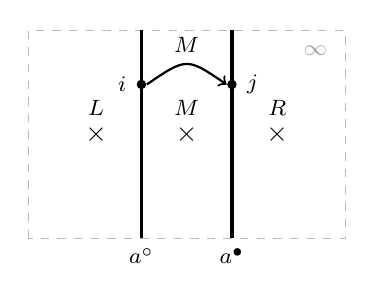
\begin{tikzpicture}[scale=1.15]
% the chart: the pillowcase with the distinguished corner sent to infinity
\draw[gray!55,dashed] (-1.75,-1.15) rectangle (1.75,1.15);
% the two generating arcs, properly embedded, both ends running to the puncture at infinity
\draw[very thick] (-0.5,-1.15) -- (-0.5,1.15);
\draw[very thick] ( 0.5,-1.15) -- ( 0.5,1.15);
\node[below] at (-0.5,-1.15) {\footnotesize $a^{\circ}$};
\node[below] at ( 0.5,-1.15) {\footnotesize $a^{\bullet}$};
% the three remaining corners, one per face
\foreach \x in {-1,0,1}{\node at (\x,0) {$\times$};}
\node[above] at (-1,0.10) {\footnotesize $L$};
\node[above] at ( 0,0.10) {\footnotesize $M$};
\node[above] at ( 1,0.10) {\footnotesize $R$};
% one generator on each arc and the arrow between them
\fill (-0.5,0.55) circle (1.5pt);  \node[left]  at (-0.56,0.55) {\footnotesize $i$};
\fill ( 0.5,0.55) circle (1.5pt);  \node[right] at ( 0.56,0.55) {\footnotesize $j$};
\draw[->,thick] (-0.44,0.55) .. controls (0,0.85) .. (0.44,0.55);
\node[above] at (0,0.80) {\footnotesize $M$};
\node[gray!70] at (1.42,0.92) {\footnotesize $\infty$};
\end{tikzpicture}
\medskip
\caption{The chart used in Section~\ref{sec:typeD}. The distinguished pillowcase corner is sent to
infinity, leaving the other three corners ($\times$) in the plane. The two generating arcs
$a^{\circ},a^{\bullet}$ are properly embedded and cut the chart into three faces, one per remaining
corner, labelled $L$, $M$ and $R$. A generator is an intersection of a curve with $a^{\circ}$ or
$a^{\bullet}$, and carries the corresponding idempotent; a segment running from $i$ to $j$ through
the face $X$ contributes an arrow $i\xrightarrow{X^{k}}j$, where $k$ counts the crossings of the
arcs. Faces $L$ and $R$ have both endpoints on the same arc, so their words join generators of equal
idempotent; $M$ joins the two arcs.}
\label{fig:chart}
\end{figure}

\subsection{The two explicit twisted complexes}
Translate the distinguished corner $(0,\pi)$ to the point at infinity of the chart.
The $q=7$ blue curve then meets the arc system in 74 points of the torus cover, that is in 37
points of the pillowcase, each with two lifts.  Three unit cancellations leave the following
31-generator complex $N$.  Its $\iota_\circ$ generators are
\[
 V_N^\circ=\{1,2,5,6,15,16,20,21,32,33\},
\]
and the remaining generators in
\begin{multline*}
 V_N=\{0,1,2,3,4,5,6,7,8,9,10,13,14,15,16,17,18,19,\\
       20,21,22,23,26,27,30,31,32,33,34,35,36\}
\end{multline*}
carry $\iota_\bullet$.  The differential is
\begin{align*}
\delta_N={}&
17\xrightarrow R18+16\xrightarrow M17+16\xrightarrow L15
+15\xrightarrow M14+14\xrightarrow R13+13\xrightarrow{M^2}10\\
&+10\xrightarrow R9+8\xrightarrow{M^2}9+7\xrightarrow R8
+6\xrightarrow M7+6\xrightarrow L5+5\xrightarrow M4+4\xrightarrow R3\\
&+2\xrightarrow M3+2\xrightarrow L1+1\xrightarrow M0+0\xrightarrow R19
+20\xrightarrow M19+20\xrightarrow L21+21\xrightarrow M22\\
&+22\xrightarrow R23+23\xrightarrow{M^2}26+26\xrightarrow R27
+30\xrightarrow{M^2}27+31\xrightarrow R30+32\xrightarrow M31\\
&+32\xrightarrow L33+33\xrightarrow M34+34\xrightarrow R35
+35\xrightarrow{M^2}36.
\end{align*}
Here and below an omitted exponent is one.  Direct path multiplication gives $\delta_N^2=0$.

The red earring curve meets the arc system in eight points.  One unit cancellation leaves a six-generator
complex $\mathcal E$ with $\iota_\circ$ generators $5,6$, $\iota_\bullet$ generators $0,3,4,7$, and
\begin{equation}\label{eq:red-typeD}
 \delta_{\mathcal E}=3\xrightarrow{M^2}0+4\xrightarrow R3+5\xrightarrow M4
 +6\xrightarrow L5+6\xrightarrow M7+0\xrightarrow R7.
\end{equation}
Again $\delta_{\mathcal E}^2=0$.

\subsection{Local reconnections and four geometric deformations}
The cross-resolution presents the blue curve as the union of the strands inherited from the
abelian fiber product and the short connector arcs inserted at the seam circles.  We call a
self-intersection \emph{connector--main} if one branch is a connector and the other is an inherited
strand, and \emph{connector--connector} if both branches are connectors.  The \emph{alternate local smoothing} at a self-intersection orbit replaces the original passage by
the other pairing, in disjoint disks around its two involution-related torus lifts.  We call the
resulting four-arrow element $b_s\in\operatorname{End}(N)$ the \emph{switch} at $s$.  We call the smoothing \emph{generator-preserving} if,
after the three standard unit cancellations, its type-D encoding has the same idempotent module
$V_N$ as $N$.  In that case its differential differs from $\delta_N$ by a four-arrow switch.

The four geometric self-intersection orbits used below are listed in the original pillowcase coordinates:
\begin{center}
\begin{tabular}{c|c}
self-intersection & $(\gamma,\theta)$ \\ \hline
$S_{18}$ & $(0.0304313,4.5024806)$ \\
$S_{25}$ & $(3.0828526,1.7672244)$ \\
$S_{69}$ & $(0.0415966492,5.4053953343)$ \\
$S_{74}$ & $(3.079988,3.561056)$
\end{tabular}
\end{center}
At each of these, perform the same local pairing at its two involution-related torus lifts.  The smoothing is
disjoint from the arc system, so the smoothed and unsmoothed complexes have the same generators after
the cancellations above.  Only two arrows change.  Define $b_s$ to be the sum of the two old and two
new arrows in the following table.
The final column records the relative word length $\deg_w$ determined by the standard KWZ grading
and $\delta_N$; it is not used in the Maurer--Cartan or wrapped-rank calculation.
\begin{center}
\small
\begin{tabular}{c|c|c|c}
$s$ & old arrows & new arrows & $\deg_w$ of the four terms \\ \hline
$S_{18}$ & $4\xrightarrow R3,\ 22\xrightarrow R23$
 & $22\xrightarrow R3,\ 4\xrightarrow R23$ & $-8,0,0,8$ \\
$S_{25}$ & $6\xrightarrow L5,\ 20\xrightarrow L21$
 & $20\xrightarrow L5,\ 6\xrightarrow L21$ & $-8,0,0,8$ \\
$S_{69}$ & $0\xrightarrow R19,\ 26\xrightarrow R27$
 & $0\xrightarrow R27,\ 26\xrightarrow R19$ & $-8,0,0,8$ \\
$S_{74}$ & $20\xrightarrow L21,\ 32\xrightarrow L33$
 & $20\xrightarrow L33,\ 32\xrightarrow L21$ & $-4,0,0,4$
\end{tabular}
\end{center}
Every displayed arrow has relative delta degree $-1$.  The auxiliary-degree columns show why none of
the four deformations belongs to the bigraded subcategory; this is immaterial for the ungraded
statement of Proposition~\ref{prop:q7-typeD}.

\begin{proof}[Proof of Proposition~\ref{prop:q7-typeD}]
For each row of the table, multiplication in $\mathcal B$ gives separately
\[
 D_N(b_s)=0,\qquad b_s^2=0.
\]
The two old and two new arrows have pairwise matching sources and targets, so pre- and
post-composition with $\delta_N$ produce cancelling pairs over $\F_2$; and $b_s^2=0$ because no
two of the four arrows compose.
Thus \eqref{eq:typeD-MC} holds.  Direct encoding of the locally smoothed curve gives
$\delta_{N_s}=\delta_N+b_s$ entry by entry, rather than merely producing a quasi-isomorphic complex.
The torus component classes and the dimensions of the two projected summands are
\begin{center}
\begin{tabular}{c|c|c}
$s$ & oriented torus component classes & wrapped summand dimensions \\ \hline
$S_{18}$ & $(2,2),(-17,-6),(-2,-2)$ & $4+5$ \\
$S_{25}$ & $(2,2),(-17,-6),(-2,-2)$ & $4+5$ \\
$S_{69}$ & $(17,8),(-2,-1),(-2,-1)$ & $5+4$ \\
$S_{74}$ & $(15,8),(-3,-1),(-3,-1)$ & $7+2$.
\end{tabular}
\end{center}
The two involution-related torus components in each three-component row project to one pillowcase
component and are counted once.

The wrapped morphism calculation uses the full positive path algebra, not a word cutoff:
Lemma~\ref{lem:wrapped-reduction} reduces it to the three numbers $e$, $\tau$, $r$ of
\eqref{eq:wrapped-reduction}.  Carrying out that reduction gives the following data.
\begin{center}
\begin{tabular}{c|c|c|c|c}
object or component & $e$ & $\tau$ & $r$ & $e+\tau-2r$ \\ \hline
$N$ & $104$ & $105$ & $101$ & $7$ \\
$N_{S_{18}}^{(1)}$ & $24$ & $20$ & $20$ & $4$ \\
$N_{S_{18}}^{(2)}$ & $80$ & $85$ & $80$ & $5$ \\
$N_{S_{25}}^{(1)}$ & $24$ & $20$ & $20$ & $4$ \\
$N_{S_{25}}^{(2)}$ & $80$ & $85$ & $80$ & $5$ \\
$N_{S_{69}}^{(1)}$ & $84$ & $85$ & $82$ & $5$ \\
$N_{S_{69}}^{(2)}$ & $20$ & $20$ & $18$ & $4$ \\
$N_{S_{74}}^{(1)}$ & $76$ & $75$ & $72$ & $7$ \\
$N_{S_{74}}^{(2)}$ & $28$ & $30$ & $28$ & $2$
\end{tabular}
\end{center}
Equation~\eqref{eq:wrapped-reduction} therefore gives the undeformed dimension seven and the four
deformed dimensions nine.  This proves the proposition.
\end{proof}

\begin{remark}
The encoding does not depend on the size of the disks in which the smoothing is performed: at radii
$0.003$, $0.006$ and $0.009$ in the displayed pillowcase coordinates the four four-arrow elements and
all of the morphism dimensions agree.
\end{remark}

\begin{corollary}\label{cor:q7-classes}
The four deformations in Proposition~\ref{prop:q7-typeD} represent exactly three
homotopy-equivalence classes in $\operatorname{Tw}(\mathcal B)$.  The $S_{18}$ and $S_{25}$ objects
are strictly isomorphic.  Their common class, the $S_{69}$ class, and the $S_{74}$ class are pairwise
distinct.
\end{corollary}

\begin{proof}
The idempotent-preserving permutation
\[
 (4\ 22)(5\ 21)
\]
and the identity on the other 27 generators carries
$\delta_N+b_{S_{18}}$ entry by entry to $\delta_N+b_{S_{25}}$.

For the converse, record the homology classes in the torus double cover of the two projected
components, with each class taken up to sign.  The three resulting multisets are
\[
 \{(2,2),(17,6)\},\qquad
 \{(2,1),(17,8)\},\qquad
 \{(3,1),(15,8)\}
\]
for $S_{18}/S_{25}$, $S_{69}$, and $S_{74}$, respectively.  These multisets are invariant under
regular homotopy in the punctured pillowcase.  The immersed-curve classification identifies
homotopy-equivalence classes of twisted complexes over $\mathcal B$ with regular-homotopy classes of
decorated immersed curves \cite[\S11.5]{CHKK}.  The three objects are therefore pairwise not
homotopy equivalent.
\end{proof}

\begin{hypothesis}[$q=7$ local support]\label{hyp:q7-support}
If the CHKK tangle assignment is defined for $Q_{1/3}+Q_{1/7}$, its curved object is homotopy
equivalent either to $(N,b_s)$ for one of the 45 distinct switches obtained by a
generator-preserving singleton smoothing at any self-intersection orbit of the PL curve, or to
$(N,b)$ for an element
\[
 b\in\operatorname{span}_{\F_2}
 \{b_{S_{18}},b_{S_{25}},b_{S_{69}},b_{S_{74}}\}.
\]
\end{hypothesis}

\subsection{Selection by a second closure}
Rank nine alone does not determine the object: by Corollary~\ref{cor:q7-classes} three homotopy
classes achieve it.  The remedy is to pair the same tangle against a \emph{second} closure, whose
instanton rank is computed by running the argument of Theorem~\ref{thm:inat} a second time.  Two
matching dimensions are a sharper constraint than one.

\begin{proposition}[The second closure separates the three classes]\label{prop:aux-closure}
Set
\[
 K_*:=\operatorname{num}(Q_{-3/4}+Q_{1/3}+Q_{1/7}).
\]
Then $\dim_{\F_2}I^\natural(K_*;\F_2)=31$.  Encoding the piecewise-linear curve of the rational earring tangle $\widehat Q_{-3/4}$ as in
Section~\ref{sec:typeD} gives a twisted complex $\mathcal E_*$.  Its wrapped morphism dimensions with the three
classes of Corollary~\ref{cor:q7-classes} are $31$, $23$ and $25$, for $S_{18}/S_{25}$, $S_{69}$
and $S_{74}$ respectively.
\end{proposition}

\begin{proposition}[Smoothings at a single orbit: an exhaustive enumeration]\label{prop:aux-selection}
The resolved blue curve has 82 self-intersection orbits: 52 are connector--main and
30 are connector--connector.  Among the 82 alternate local smoothings, 73
are generator-preserving.  They determine 45 distinct, linearly independent four-arrow
elements $b_s\in\operatorname{End}(N)$, and every one satisfies
\[
 D_N(b_s)=0,\qquad b_s^2=0.
\]
Among all 73 occurrences, the simultaneous wrapped dimensions nine against the
original rational earring $\mathcal E$ and 31 against $\mathcal E_*$ occur only at $S_{18}$ and $S_{25}$.
They are also the only generator-preserving occurrences whose shorter branch loop has absolute torus
deck class $(2,2)$.
\end{proposition}

\begin{proposition}[How far the two-closure constraint reaches]\label{prop:aux-span}
Every element
\[
 b=\epsilon_{18}b_{S_{18}}+\epsilon_{25}b_{S_{25}}
   +\epsilon_{69}b_{S_{69}}+\epsilon_{74}b_{S_{74}},
 \qquad \epsilon_s\in\F_2,
\]
is Maurer--Cartan.  Among these 16 deformations, the simultaneous wrapped dimensions nine
against the original rational earring and 31 against $\mathcal E_*$ occur only for
$b=b_{S_{18}}$ and $b=b_{S_{25}}$.

The selector does not reach further.  The connector--main subcensus consists of 46 occurrences and
38 distinct switches.  Every one of the $\binom{38}{2}=703$ sums of two distinct switches in this
subcensus is Maurer--Cartan.  The 38 elements are linearly independent, so all $2^{38}$ elements of
their $\F_2$-span are distinct and Maurer--Cartan.  Of the two-switch sums, 41 also have
wrapped-dimension pair $(9,31)$.  None of these 41 presentations is carried to the
$S_{18}$ presentation by an idempotent-preserving permutation of the 31 generators.
\end{proposition}

\begin{corollary}[Conditional selection]\label{cor:aux-conditional}
Assume the CHKK instanton--pillowcase correspondence and Hypothesis~\ref{hyp:q7-support}.  Then the
object assigned to $Q_{1/3}+Q_{1/7}$ is homotopy equivalent to the common $S_{18}/S_{25}$ class.
\end{corollary}

\begin{proof}[Proof of Propositions~\ref{prop:aux-closure}--\ref{prop:aux-span} and
Corollary~\ref{cor:aux-conditional}]
The knot $K_*$ has the 14-crossing planar diagram
\[
\begin{aligned}
&(24,13,25,14),\ (10,25,11,26),\ (26,11,27,12),\ (12,27,13,0),\ (7,14,8,15),\\
&(15,8,16,9),\ (9,16,10,17),\ (23,6,24,7),\ (5,22,6,23),\ (21,4,22,5),\\
&(3,20,4,21),\ (19,2,20,3),\ (1,18,2,19),\ (17,0,18,1),
\end{aligned}
\]
in the usual $PD$ convention, so the calculation below can be repeated in any standard package.
Seifert's algorithm applied to it gives
\[
\begin{aligned}
 \Delta_{K_*}(t)={}&t^{-6}-t^{-5}+2t^{-3}-4t^{-2}+5t^{-1}-5\\
 &+5t-4t^2+2t^3-t^5+t^6.
\end{aligned}
\]
Thus $\ell(K_*)=31$ and $|\Delta_{K_*}(-1)|=23$.  Over $\F_2$, the reduced Khovanov dimensions in
homological degrees zero through 13 are
\[
 (1,0,1,1,1,2,3,3,4,5,4,3,2,1),
\]
whose sum is $31$; this is a finite computation from the diagram above, reproducible in any Khovanov package.  The Alexander lower bound, universal coefficients, and the reduced
Khovanov-to-instanton spectral sequence therefore give
\[
 31=\ell(K_*)
 \le \dim_{\Q}I^\natural(K_*;\Q)
 \le \dim_{\F_2}I^\natural(K_*;\F_2)
 \le \dim_{\F_2}\widetilde{Kh}(K_*;\F_2)=31.
\]

For the algebraic pairing, the reduction data $(e,\tau,r,e+\tau-2r)$ of
Equation~\eqref{eq:wrapped-reduction} are
\[
\begin{array}{c|rrrr}
\text{blue class} & e&\tau&r&e+\tau-2r\\ \hline
S_{18}/S_{25}&228&251&224&31\\
S_{69}&228&251&228&23\\
S_{74}&228&251&227&25.
\end{array}
\]
These are all-word computations in $\operatorname{Tw}(\mathcal B)$.  Under the stated
correspondence, the rational-earring cochains vanish \cite[Lem.~5.3]{Smith}.

For the exhaustive local census, retaining the provenance of each segment partitions the
82 self-intersection orbits into 52 connector--main and 30 connector--connector orbits.  The
alternate equivariant smoothing is encoded directly at every orbit.  The nine nodes
\[
 S_7,S_8,S_{23},S_{24},S_{49},S_{52},S_{53},S_{61},S_{73}
\]
change the cancelled module.  At every other node the symmetric difference of the two
differentials consists of two old and two new arrows.  Exact path multiplication gives
$D_N(b_s)=b_s^2=0$ in every case.  Duplicate node presentations leave 45 distinct elements,
and expanded in the basis of arrows, the 45 elements are linearly independent.  Applying the
mapping-cone reduction
\eqref{eq:wrapped-reduction} to both rational earrings gives the complete census
\[
\begin{array}{c|rr}
(\dim H\operatorname{Mor}(\mathcal E,(N,b_s)),
  \dim H\operatorname{Mor}(\mathcal E_*,(N,b_s)))
 &\text{self-intersection orbits}&\text{distinct switches}\\ \hline
(5,23)&1&1\\
(5,25)&2&2\\
(7,23)&12&6\\
(7,25)&39&23\\
(7,27)&8&4\\
(9,23)&1&1\\
(9,25)&8&6\\
(9,31)&2&2
\end{array}
\]
The final row consists precisely of $S_{18}$ and $S_{25}$.  For each node, the two arcs between its
preimages determine complementary branch loops.  Choosing the loop with smaller $\ell^1$ deck norm
and forgetting signs gives an additional finite label; $(2,2)$ occurs among the 73
generator-preserving occurrences only at the same two nodes.

Restricting to connector--main nodes recovers 46 generator-preserving occurrences and
38 distinct switches.  Expanded in the basis of arrows, those 38 are linearly independent.  For
each unordered pair of these distinct switch elements, exact multiplication verifies the
Maurer--Cartan equation for their sum.  Since the individual elements are closed and square-zero,
the pair checks say exactly that all mixed anticommutators vanish.  Every one of their $2^{38}$ sums
is therefore Maurer--Cartan.
Applying the same two mapping-cone reductions to all $\binom{38}{2}=703$ two-switch sums gives
41 sums with rank pair $(9,31)$.  Thus the two
closure dimensions select the singleton class but do not select within the unrestricted span of
local switches.  For a presentation-level comparison, regard each differential as a directed graph
on the 31 generators whose vertices carry their idempotents and whose edges retain their face and
path length.  An exhaustive search over the bijections preserving all of that data finds none
carrying the $S_{18}$ differential to any of the 41; the same search does find the
$S_{18}$--$S_{25}$ permutation, which is known independently.  This distinguishes strict
presentations only; it is not a claim that the 41 objects are pairwise inequivalent up to homotopy.

Direct multiplication also shows that every sum of the four named switches satisfies the
Maurer--Cartan equation.  Of the 16 deformations, eight have original-closure dimension nine;
their auxiliary dimensions are
\[
\begin{array}{c|c}
b&\dim H\operatorname{Mor}(\mathcal E_*,(N,b))\\ \hline
b_{S_{18}},\ b_{S_{25}}&31\\
\substack{b_{S_{69}},\ b_{S_{18}}+b_{S_{25}}+b_{S_{69}},\\
 b_{S_{25}}+b_{S_{69}}+b_{S_{74}},\\
 b_{S_{18}}+b_{S_{25}}+b_{S_{69}}+b_{S_{74}}}&23\\
b_{S_{74}},\ b_{S_{18}}+b_{S_{74}}&25.
\end{array}
\]
The other eight sums have original-closure dimension seven.  Pairing the assigned object with the
original and auxiliary rational earrings must recover dimensions nine and 31, respectively.
In either of the two stated localization classes, the displayed censuses leave only $b_{S_{18}}$
and $b_{S_{25}}$, whose objects are strictly isomorphic by Corollary~\ref{cor:q7-classes}.
\end{proof}

\begin{remark}\label{rem:q7-scope}
Proposition~\ref{prop:q7-typeD} proves existence of four named Maurer--Cartan elements, and
Proposition~\ref{prop:aux-selection} proves the exhaustive singleton census in the stated geometric
class; neither proposition proves selection by the tangle.  Indeed, the ungraded delta-degree
$-1$ endomorphism cohomology of $N$ is much larger than its one-dimensional auxiliary-degree-zero
part.  Corollary~\ref{cor:q7-classes} shows concretely that the wrapped-rank match leaves three
different homotopy-equivalence classes.  The auxiliary closure strengthens selection both to every
generator-preserving singleton smoothing at any PL node and to all 16 sums of the four named
switches, but only after assuming the CHKK correspondence and that its assigned object is represented
in one of these stated classes.  The algebraic calculation proves neither assumption.
The restriction on support is essential: Proposition~\ref{prop:aux-span} exhibits 41
two-switch sums outside the singleton statement with the same two closure dimensions.
\end{remark}

\subsection{A two-generator Yoneda reduction}
There is a formal recognition alternative to identifying the virtual chain of every figure-eight
bubble, although the available wrapped representability theorem will not apply below.  In the
compact setting, Fukaya proves that an unobstructed immersed Lagrangian correspondence with clean
geometric composition produces a canonical gauge-equivalence class of bounding cochain on the
composition, and that the resulting object represents the quilted correspondence module
\cite[Thms.~6.3 and~7.3]{FukayaCorr}.  Gao proves the corresponding representability statement for
properly embedded exact cylindrical correspondences between Liouville manifolds
\cite[Thm.~7.24 and Cor.~7.25]{Gao}, on the unobstructedness input of \cite[Thm.~7.12]{Gao}.  These theorems obtain the output object by a cyclic-element and
Yoneda argument; they do not require the still-open identification of its cochain with a virtual
chain of figure-eight bubbles.  Proposition~\ref{prop:partial-triple}, however, shows that Gao's
embedded-correspondence hypothesis fails in the present geometry.

Let $\mathcal C\subset\mathcal W(P^*)$ be the CHKK full subcategory of unobstructed objects missing
the top-left puncture, let $G=a^\circ\oplus a^\bullet$, and let
$\mathcal B=\operatorname{End}_{\mathcal C}(G)$.  Thus $G$ split-generates $\mathcal C$ and
$\mathcal C\simeq\operatorname{Tw}(\mathcal B)$ \cite[\S11.5]{CHKK}.

\begin{proposition}[Two-generator Yoneda recognition]\label{prop:yoneda-recognition}
Assume that the quilted module
\[
 \mathcal M_{F_{1/3,t}}(A_{1/7})
\]
is defined and is represented by an object $X_{1/3,1/7}\in\mathcal C$.  If there is an
$A_\infty$ quasi-isomorphism of right
$\mathcal B$-modules
\[
 \mathcal M_{F_{1/3,t}}(A_{1/7})\big|_{\mathcal B}
 \simeq
 \operatorname{Mor}_{\operatorname{Tw}(\mathcal B)}
       \bigl(G,(N,b_{S_{18}})\bigr),
\]
then
\[
 X_{1/3,1/7}\simeq (N,b_{S_{18}})\simeq(N,b_{S_{25}})
 \qquad\text{in }\mathcal C.
\]
It is enough to specify the module on the two objects $a^\circ,a^\bullet$, but this means the full
chain-level complexes together with every $\mathcal B$-action and higher module map.  Homology
dimensions of pairings with two test objects do not imply the conclusion.
\end{proposition}

\begin{proof}
The $A_\infty$ Yoneda embedding is cohomologically fully faithful.  Since $G$ split-generates
$\mathcal C$, restricted Yoneda is cohomologically fully faithful on $\mathcal C$, and its
split-closed triangulated envelope is the category of perfect $\mathcal B$-modules.
Representability identifies the first module in the display with the Yoneda module of
$X_{1/3,1/7}$.  The assumed module quasi-isomorphism is consequently the Yoneda image of a
homotopy equivalence
$X_{1/3,1/7}\simeq(N,b_{S_{18}})$.  The second equivalence is the strict isomorphism of
Corollary~\ref{cor:q7-classes}.

The last assertion records what restriction to the two-object category $\mathcal B$ entails.  The
closure dimensions in Proposition~\ref{prop:aux-closure} retain only the dimensions of two module
homologies.  Its 41 two-switch collisions show directly that those dimensions do not recover
the module or the represented object.
\end{proof}

\section{Finite polygon counts, and what a genuine deformation would require}\label{sec:combinatorial}

\subsection{A finite winding test}\label{ss:polygons}
For two transverse embedded loops on an oriented surface, de~Silva--Robbin--Salamon identify
holomorphic strips with combinatorial lunes under precise hypotheses \cite{dSRS}.  Those hypotheses
do not cover the present calculation: the curves are immersed, the pillowcase has orbifold points,
and a bounding-cochain deformation uses higher polygons.  Accordingly, this section defines only a
finite combinatorial test, and records what it does not decide.

For intersection points $x,y$, choose an arc $\alpha$ on red from $x$ to $y$ and an arc $\beta$ on
blue from $y$ to $x$, and lift the loop $\Gamma=\alpha\cdot\bar\beta$ to the torus.  The pair is
accepted as a candidate bigon when (a) the lifted loop is null-homologous; (b) its winding function
is zero at the four pillowcase corners; (c) that function is nonnegative on the sampled complementary
regions; and (d) the local sectors at $x$ and $y$ are convex.  The same conditions at every vertex
define the candidate triangle and quadrilateral tables.  We refer to the conjunction of these
conditions as the \emph{low-order test}, and we call the set of self-intersections at which the
tabulated windows contain a complete polygon the \emph{active set}.  Both are finite combinatorial
conditions, not a theorem that all and only analytic polygons have been counted.

The matrices use one fixed lift of the red curve and sum over the two torus preimages of a blue
self-intersection; the crossings carry the enumeration fixed by that construction, and it is this
enumeration that the positions quoted in Section~\ref{sec:compute} refer to.  Candidate arcs are
restricted by explicit edge-index windows.  The triangle count, too, uses finite blue and red
spans.  No geometric
bound proves these windows exhaustive, and the bigon count considers only single traversals of the
chosen arcs.  Multiple-wrapping lunes and polygons are not enumerated.  These limitations are why
the outputs in Section~\ref{sec:compute} are finite tables rather than Fukaya operations.

For the decomposition \eqref{eq:family} take $T_1=\Qh{-1/2}$ and
$T_2=Q_{1/3}+Q_{1/q}$.  Section~\ref{sec:setup} constructs explicit piecewise-linear curves
$R_{\mathrm{PL}}$ and $L_{q,\mathrm{PL}}$ from Smith's fiber-product and resolution description.
For the reported perturbation parameters, let $C_q$ be the $\F_2$-vector space generated by their
transverse intersections, and let $D_q^{\mathrm{big}}$ be the matrix of the winding-number bigon
count defined in Section~\ref{ss:polygons}.  Define
\begin{equation}\label{eq:big-stat}
 h_q^{\mathrm{big}}
 :=\dim_{\F_2}C_q-2\rk_{\F_2}D_q^{\mathrm{big}}.
\end{equation}
We call this the \emph{bigon-rank statistic}.  Equation \eqref{eq:big-stat} is a definition for a
finite matrix.  It does not, by itself, assert that $D_q^{\mathrm{big}}$ is the differential of an
analytic or invariant Floer complex.

\subsection{What the full deformation would require}\label{ss:deformed}
At a transverse self-intersection $p$ of an immersed curve, immersed Floer theory has two ordered
branch-jump generators, one for each ordering of the preimages; in a graded setup their degrees are
complementary \cite{AkahoJoyce}.  A geometric double point without an ordering is therefore not an
algebraic generator.  If $b$ is a degree-one element in an appropriate completed curved $A_\infty$ algebra,
the Maurer--Cartan equation is the full series \eqref{eq:MC}.  For two objects carrying cochains
$b_0,b_1$, the deformed morphism differential has the form
\begin{equation}\label{eq:defdiff}
 d_{b_1,b_0}(x)=
 \sum_{r,s\ge0}\mu^{r+s+1}(b_1^{\otimes r},x,b_0^{\otimes s}),
\end{equation}
up to the convention for the order of boundary inputs.  Thus both formulas contain ordered words,
allow repeated occurrences of the same branch jump, and have no a priori upper bound on word
length.  A positive Novikov filtration or a geometric nilpotence statement is also needed to define
the infinite sums.

The finite tables below are coarser.  They label the underlying double point rather than an
ordered branch jump.  Its displayed deformation includes bigons, triangles, and quadrilaterals
through distinct selected crossings, stored as sets; the accompanying Maurer--Cartan test uses the
tabulated monogon and self-bigon terms and selected distinct-input self-triangles.  In
particular, it omits repeated terms and all uncontrolled higher words.  An empty monogon
table is a finite output, not a proof that $\mu^0$ vanishes.  Nor does a degree argument dispose of
the question: without a proved grading and phase bound, self-intersection generators need not be
confined to degrees zero and one.

For genuine solutions of the full Maurer--Cartan equation, the curved $A_\infty$ relations imply
$d_{b_1,b_0}^2=0$.  Therefore square-zero is a necessary check on any proposed finite
matrix.  It is not sufficient: a square-zero truncation may still omit terms in \eqref{eq:defdiff}.

\section{Finite candidate supports at $q=5,7,11$}\label{sec:compute}

\begin{computation}[Finite bigon-rank pattern]\label{comp:law}
For the specified representatives and parameters, the counts are
\[
 h_5^{\mathrm{big}}=5,\qquad h_7^{\mathrm{big}}=7,\qquad
 h_{11}^{\mathrm{big}}=15,\qquad h_{13}^{\mathrm{big}}=17.
\]
The raw bigon matrices checked at $q=5,7,11,13$ square to zero over $\F_2$.  The value $5$ at $q=3$ in
Table~\ref{tab:family} is instead the published computation of \cite[\S11.6]{HHK2}, made from a
different tangle presentation; it is not an output of this uniform piecewise-linear family.
\end{computation}

\begin{table}[ht]
\centering
\small
\begin{tabular}{c|ccccc}
 $q$ & $\det K_q$ & bigon statistic & $\dim_{\F_2}\Inat$ & difference & required matrix-rank change \\ \hline
 $3$ & $3$ & $5$ (external) & $5$ & $0$ & $0$ \\
 $5$ & $1$ & $5$ & $7$ & $-2$ & $-1$ \\
 $7$ & $1$ & $7$ & $9$ & $-2$ & $-1$ \\
 $11$ & $5$ & $15$ & $13$ & $+2$ & $+1$ \\
 $13$ & $7$ & $17$ & $15$ & $+2$ & $+1$ \\
\end{tabular}
\medskip
\caption{A finite numerical pattern.  The instanton column is unconditional by
Theorem~\ref{thm:inat}.  The bigon-statistic column for $q\ge5$ concerns the specified finite
piecewise-linear matrices; the $q=3$ entry is external.  The last column is the change in matrix rank
that would be required if a genuine deformed differential existed on the same generator module.}
\label{tab:family}
\end{table}

At these five displayed values the numerical differences satisfy
\[
 h_q^{\mathrm{big}}-(q+2)=2\,\sgn\bigl(|q-6|-3\bigr),
\]
where the left side at $q=3$ uses the external entry.  This is a finite-sample observation, not a
theorem or conjectural identification of $h_q^{\mathrm{big}}$ with Floer homology.

The matrix-rank comparison suggests looking for self-intersections at which low-order polygon terms
change the rank of $D_q^{\mathrm{big}}$ by one.  We call a finite set of self-intersections a
\emph{support}, by analogy with the set on which a cochain would be nonzero.  This search must be distinguished from solving the
full Maurer--Cartan equation.  For a finite set $S$ of self-intersections, define
$D_q^{\mathrm{tab}}(S)$ by adding to $D_q^{\mathrm{big}}$ the tabulated triangle terms and the
tabulated quadrilateral terms through \emph{distinct} crossings of $S$, and record
\begin{equation}\label{eq:tab-stat}
 h_q^{\mathrm{tab}}(S):=\dim_{\F_2}C_q-2\rk_{\F_2}D_q^{\mathrm{tab}}(S).
\end{equation}
Repeated insertions and unrestricted higher operations are absent from this definition.

\begin{computation}[Low-order candidate supports]\label{comp:cochains}
The finite search gives the following outputs.
\begin{enumerate}
\item[(i)] At $q=5$, among the singleton and two-element subsets of the active set of
Section~\ref{ss:polygons},
the unique smallest support with $h_5^{\mathrm{tab}}=7$ is $S=\{s_A,s_B\}$, where
$(\gamma,\theta)\approx(0.03,1.27)$ and $(3.06,4.98)$.  One tabulated quadrilateral changes the
$(x_4,y_6)$ bigon entry from $0$ to $1$.  The resulting matrix has the sole entry $(x_1,y_0)$ and squares to zero.
\item[(ii)] At $q=7$, among the tested singleton crossings passing the low-order test of
Section~\ref{ss:polygons},
one crossing near $(0.05,5.41)$ has $h_7^{\mathrm{tab}}=9$.  Its tabulated triangle changes one bigon entry
from $1$ to $0$.  The resulting matrix has entries $(6,4)$ and $(7,5)$ and squares to zero.
\item[(iii)] At the default $q=11$ perturbation, 55 singleton crossings pass the
low-order test and have matrix rank three.  Exactly 52 of the resulting
matrices square to zero.  Three of the 55 do not: their squares
have respective nonzero entries $(9,15)$, $(9,14)$, and $(0,14)$.  At the independent parameter
choice $(\varepsilon_{\rm blue},\varepsilon_{\rm red},r_{\rm red})=(0.03,0.10,0.25)$, the same
test returns 56 singleton candidates of the target rank; 14 matrices fail square-zero,
leaving 42 that pass this necessary condition.
\end{enumerate}
\end{computation}

A geometric double point gives two ordered
branch-jump generators; in a graded immersed setup their degrees are complementary.  The original
search stores only the underlying geometric crossing.  Moreover, the test uses only the tabulated
monogon, self-bigon, and distinct-crossing self-triangle terms.  It does not test the full series \eqref{eq:MC}.  Therefore
Computation~\ref{comp:cochains} proves neither existence nor uniqueness of a bounding cochain.

\subsection{$q=5$: a quadrilateral in the finite table}\label{ss:b5}
The raw bigon matrix has rank two.  Within the active set, no singleton and exactly
one tested two-element support lowers the tabulated matrix rank to one.  It consists of the crossings
$s_A,s_B$ in Figure~\ref{fig:pillow}.  The accepted quadrilateral changes the $(x_4,y_6)$ entry, so
the tabulated matrix retains only $(x_1,y_0)$, squares to zero, and has
$h_5^{\mathrm{tab}}=9-2=7$.  This proves the finite statement in
Computation~\ref{comp:cochains}(i), including minimality only within the stated active-set search.
It does not prove that the two unoriented crossings define a degree-one element, solve the full
Maurer--Cartan equation, or give the full differential \eqref{eq:defdiff}.

\subsection{$q=7$: a triangle in the finite table}\label{ss:b7}
The raw bigon matrix has rank three.  At the default parameters, one tested singleton near
$(0.042,5.405)$ passes the low-order test and its accepted triangle lowers the
tabulated rank to two.  The resulting entries are $(6,4)$ and $(7,5)$; the matrix squares to zero and
$h_7^{\mathrm{tab}}=13-4=9$.  At the second parameter choice the corresponding crossing is near
$(0.058,5.413)$ and again gives a rank-two square-zero table, although its generator labels and
entries change.  This is the finite statement in Computation~\ref{comp:cochains}(ii), not a full
Maurer--Cartan calculation.  The crossing is $S_{69}$ in the labeling of
Section~\ref{sec:typeD}.  Its type-D deformation is the four-arrow switch $b_{S_{69}}$, not the
single untyped support used by this finite table.

\subsection{$q=11$: three tables fail the square-zero condition}\label{ss:b11}
At the default parameters $(\varepsilon_{\rm blue},\varepsilon_{\rm red},r_{\rm red})=(0.05,0.16,0.40)$
the raw bigon matrix has 19 generators and rank two.  The
unoriented, low-order test returns 55 singleton supports whose tabulated matrices have rank
three.  Three of the 55 fail the necessary square-zero condition, with the nonzero square entries listed in
Computation~\ref{comp:cochains}(iii).  So 55 is not a count of
differentials or of bounding cochains, even inside the truncation.

The count is also parameter-dependent.  At
$(\varepsilon_{\rm blue},\varepsilon_{\rm red},r_{\rm red})=(0.03,0.10,0.25)$, the raw matrix has
23 generators and rank four, and the same low-order test returns 56 target-rank
singletons.  Of their matrices, 14 fail square-zero, leaving 42 that pass this necessary
test.  Neither 52 at the default parameters nor 42 at the second parameters is a count
of bounding cochains: none has been checked in the typed, full $A_\infty$ algebra.

\subsection{Smoothing evidence at $q=5,7$}
The ancillary smoothing computation resolves both local sectors at the selected $q=5$ and $q=7$
nodes and recounts accepted bigons.  For one sector choice it reproduces the corresponding tabulated
matrices entry by entry.  At $q=5$ this remains a finite single-traversal test.  At $q=7$,
Proposition~\ref{prop:q7-typeD} replaces the smoothing experiment by a full algebraic calculation:
the direct smoothing is encoded over $\mathcal B$, its four-arrow difference is Maurer--Cartan, and
the wrapped pairing is computed without a word cutoff.

To turn the $q=5$ experiment into a proof one needs a surgery lemma for that immersed curve: after choosing
degree-one ordered branch jumps and smoothing them in disjoint disks, collapsing the smoothing arcs
must give a bijection between \emph{all} bigons of the smoothed pair and \emph{all} polygons in
\eqref{eq:defdiff}, including repeated visits and multiple wrapping.  One must also prove a grading
statement that makes the selected branch jumps degree one and controls every term of the full
Maurer--Cartan series.  No theorem cited here supplies those assertions for the $q=5$ curve in the
punctured orbifold pillowcase, and the present enumerator does not prove them.  At $q=7$ the type-D
calculation avoids this surgery lemma.  Corollary~\ref{cor:aux-conditional} conditionally selects
one of its three homotopy classes, but Remark~\ref{rem:q7-scope} still prevents identifying that
class with the tangle's conjectural bounding cochain unconditionally.

\section{Discussion}\label{sec:disc}

\subsection{The finite pattern}
For the five displayed rows, including the external $q=3$ row, the numerical difference between the
bigon statistic and the instanton dimension is governed by $\det K_q\gtrless3$.  This observation has
only four outputs of the uniform program behind it and is not evidence that either finite matrix is
an invariant.  In particular, one cannot presently infer a family-wide ``one differential'' law or
a theorem about the size of a bounding cochain from Table~\ref{tab:family}.  A meaningful next step
would be to construct a genuine filtered immersed Floer complex for every admissible $q$ and only
then ask whether its undeformed rank has this determinant dependence.

\subsection{Relation to prior examples}
CHKK identify a candidate correction on the earring tangle of $T(4,5)$ and explain the expected
higher-term behavior \cite[\S10]{CHKK}; their discussion does not supply a general all-orders theorem
for the present curves.  Proposition~\ref{prop:q7-typeD} supplies an all-orders algebraic calculation
for the four named $q=7$ smoothings, but not the conjectural tangle assignment.
Proposition~\ref{prop:aux-closure} uses a second closure, and Corollary~\ref{cor:aux-conditional}
conditionally selects the common
$S_{18}/S_{25}$ class from every generator-preserving singleton smoothing at any PL node and from
the sixteen-element span of the four named switches.  Smith proves,
conditional on the CHKK correspondence, that a nonzero
cochain is required on the Conway-sum side of $P(-2,3,5)$ \cite[Thm.~5.9]{Smith}, but does not identify
it.  The $q=5$ tabulated quadrilateral is compatible with that picture but does not establish a full
correction.  The $q=11$ finite tables cannot support an analogous creation claim: three of them
fail square-zero, the surviving count is parameter-dependent, and the full deformation is unknown.

\subsection{The remaining $q=7$ localization statement}
Proposition~\ref{prop:smith-main} identifies the underlying analytic main immersion with
$L_{7,\mathrm{PL}}$ up to regular homotopy, and Section~\ref{sec:typeD} verifies the type-D equations
without a polygon cutoff.  The remaining assertion needed by the closure argument is exactly
Hypothesis~\ref{hyp:q7-support}.  Corollary~\ref{cor:aux-conditional} proves that the CHKK
correspondence and this hypothesis together force the common $S_{18}/S_{25}$ class.

A direct proof of the local-support statement would have to identify the relevant rigid
figure-eight boundary strata, exclude simultaneous multi-node or non-reconnection support, and
intertwine their output with the alternate-reconnection morphisms in the two-arc model.  A
regular homotopy of the underlying immersion alone does not transport this decoration.
Fredholm index alone does not give the required exclusion.  In the Bottman--Wehrheim
strip-shrinking model, the predicted top boundary stratum at zero width permits any positive number
of figure-eight bubbles, and the zero-input correction is a count of Morsified figure-eight bubble
trees rather than single vertices \cite[\S\S4.2--4.4]{BottmanWehrheim}.  Thus zero input and total index zero do not force
singleton support.  Any proof of Hypothesis~\ref{hyp:q7-support} must instead use the special
geometry of the six seam neighborhoods to classify the allowed trees and prove the required
mod-two cancellations.

Proposition~\ref{prop:yoneda-recognition} gives a formal second route which avoids that
classification.  Gao's construction applies only to \emph{admissible} correspondences, that is, to
objects of $\mathcal W(P_2^-\times P_3)$: properly embedded, exact and cylindrical
\cite[Def.~6.3, Def.~7.2 and the standing convention of \S7.1]{Gao}.  The representability theorem
inherits that hypothesis \cite[Thm.~7.24 and Cor.~7.25]{Gao}, as does the unobstructedness statement
it uses as input \cite[Thm.~7.12]{Gao}, which in addition requires the target projection to be
proper.  The \emph{composition} with $A_{1/7}$ is then permitted to be an immersion with transverse
or clean self-intersections \cite[Assumption~7.10]{Gao}.  Lemma~\ref{lem:surface-reduction} proves the Lagrangian
immersion, the graph description off the seam neighborhoods, and properness of the target
projection.  Proposition~\ref{prop:partial-triple} disproves embeddedness of $F_{1/3,t}$ itself.
Thus Gao's theorem cannot be invoked for this correspondence.  The triple point obstructs a second
time if one attempts to enlarge the framework: Gao's immersed theory is stated for self-intersections
that are at most double points \cite[Def.~4.4]{Gao}.  The formal recognition statement remains useful only
after either proving a wrapped representability theorem for immersed correspondences which covers
this triple point, or replacing $F_{1/3,t}$ by an embedded correspondence and proving that the
replacement induces the same quilted module.  Neither statement is currently available.  Fukaya's
compact theorem does not apply verbatim to $P^*$, and passing to the torus double cover does not by
itself repair the problem: the compactified $C_3$ space has conical singularities over the corner
points, while the required equivariant correspondence functor and its descent to the wrapped
pillowcase category have not been constructed \cite[\S11.5]{CHKK}.

After such an immersed representability or replacement theorem, the remaining symplectic
calculation would be the full $\mathcal B$-module comparison in
Proposition~\ref{prop:yoneda-recognition}.  Zhang constructs and
proves uniqueness of a quilt lifted from each prescribed bigon on closed surfaces and explicitly
applies this mechanism to CHKK's Figure~22 \cite{Zhang1,Zhang2}.  These results do not prove that
every quilted module operation arises from such a bigon, do not determine the higher module maps,
and do not supply the punctured no-escape argument.  Thus they provide entries for the proposed
module comparison, not the comparison itself.

Standard immersed-surgery results also do not automatically settle this one-dimensional case.  In
particular, degree alone need not force the Maurer--Cartan series to vanish: the ordered
self-intersections and every possible degree-two output must first be determined in a fixed grading,
and repeated words may remain compatible with that grading.  Section~\ref{sec:typeD} carries out the
finite algebraic route for $q=7$: it encodes the curves in the two-arc model and verifies the
Maurer--Cartan identities directly.  In view of Proposition~\ref{prop:partial-triple}, the presently
shortest symplectic route is therefore the direct proof of Hypothesis~\ref{hyp:q7-support}.  An
immersed wrapped-correspondence theorem plus the module quasi-isomorphism would provide an
alternative.  A separate gauge-theoretic gate would remain: one must identify
that symplectic assignment and its closure pairing with the instanton tangle invariant.  CHKK state
this assignment as Conjecture~D \cite{CHKK}; neither Fukaya's nor Gao's correspondence theorem is an
instanton--pillowcase comparison.

\subsection{Reproducibility}
The repository calculations are pure Python (standard library).  The finite polygon programs are included as
ancillary files with this preprint.  The source-repository program
\path{pillowcase/c3_perturbed.py} verifies the corrected boundary words and the three preimages
in Proposition~\ref{prop:partial-triple}.  The $q=7$ program is
\path{pillowcase/q7_kwz.py}; it prints the type-D encodings, the four Maurer--Cartan checks, the
mapping-cone reductions, the three-radius stability checks, the strict $S_{18}$--$S_{25}$
isomorphism, and the three lifted component-class multisets.  The auxiliary-closure program
\path{pillowcase/q7_closure_probe.py} prints the full sixteen-element two-closure census,
checks every Maurer--Cartan identity, verifies the Alexander polynomial from the recorded Seifert
matrix, and records the 14-crossing planar diagram.  The exhaustive local-smoothing program \path{pillowcase/q7_quilt_census.py} classifies all 82 self-intersection orbits, directly
encodes all 82 singleton reconnections, and prints the seventy-three-row two-closure census
used in Proposition~\ref{prop:aux-selection} when run with \texttt{--all-orbit-census}.  Its final
line also records, rather than assumes, the missing analytic local-support implication; the optional
connector--main two-switch census checks all 703 pair sums and the 41 rank-pair collisions.
The closure probe's optional external check uses
Spherogram~2.4.1 and Khoca~1.5 to regenerate that diagram,
the Seifert matrix, and the reduced Khovanov rank.  The delicate numerical points of
the polygon counts (long edges under mod-$2\pi$ arithmetic, shallow-angle corners, adaptive
sampling) are documented there.  A matrix whose square is nonzero is the differential of no complex, so this check precedes every
displayed statistic; the arithmetic statistic \eqref{eq:tab-stat} remains defined even for
a matrix that fails this test.  The code, the data, and both
papers are also public at
\begin{center}
\url{https://github.com/bwuebben/pillowcase-bounding-cochain}\,.
\end{center}
The curve reconstruction is checked against Smith's $q=5$ intersection and bigon counts; the finite
predicate is exercised on the unlink prototype and synthetic teardrop/lens inputs; and the raw
bigon-rank statistics are recomputed at independent parameter choices.  These regression checks do
not prove completeness of the predicate or perturbation invariance.  The instanton dimension in
Table~\ref{tab:family} is Theorem~\ref{thm:inat} and is independent of all of this code.

\appendix

\section{Changes from version 2}\label{app:changes}

This is version~3.  It differs substantially from version~2 of July 30, 2026; the changes are listed
here in full.

\begin{enumerate}
\item \emph{The title has changed.}  Version~2 was titled ``\dots\ and computed bounding cochains in
the pillowcase''.  The present title names what is actually proved, Maurer--Cartan deformations in
the two-arc algebra, and no longer asserts a bounding cochain; item~(2) below is the corresponding
withdrawal.

\item \emph{The bounding-cochain claims of version~2 are withdrawn.}  Version~2 presented
Computation~\ref{comp:cochains} as three computed bounding cochains, a unique minimal one at $q=5$
and at $q=7$ and 55 at $q=11$, and claimed them as the first computed nonzero bounding
cochains on Conway-sum tangles and the first in the pillowcase theory acting by cancellation.  The
computation behind them evaluates a finite table of monogons, self-bigons, and triangles and
quadrilaterals through distinct crossings, inside a finite edge window, with untyped and unrepeated
insertions.  It therefore does not test the Maurer--Cartan equation \eqref{eq:MC}, and no minimality
or uniqueness statement follows from it.  Those outputs appear here as candidate supports for the
explicitly defined finite matrices of Section~\ref{sec:compute}.

\item \emph{An error in the $q=11$ computation is reported.}  Three of the 55 matrices
reported in version~2 do not square to zero over $\F_2$.  At an independent parameter choice the same
test returns 56 candidates, of which 42 square to zero.  A square-zero audit now
precedes every displayed statistic and is printed by the ancillary programs.

\item \emph{The ``deficiency law'' is restated as a finite statistic.}  What version~2 called the
naive Floer rank is the bigon-rank statistic \eqref{eq:big-stat}, a definition attached to one
specified finite matrix; the pattern across the rows of Table~\ref{tab:family} is recorded as a
finite observation about those matrices, not as a law and not as an identification with Lagrangian
Floer homology.  Version~2's Hypothesis 4.1, that the winding-number counts compute the operations
$\mu^k$, no longer supports any claim of this paper.

\item \emph{The instanton theorem is strengthened to integral coefficients.}  Theorem~\ref{thm:inat}
now gives $\Inat(P(-2,3,q);\Z)\cong\Z^{q+2}$, from Manion's integral freeness \cite{Manion} together
with the integral Kronheimer--Mrowka spectral sequence; version~2 stated the rational rank.  The
Alexander polynomials are quoted from Hironaka's theorem \cite{Hironaka} rather than derived by the
skein recursion of version~2, which survives only as an ancillary regression check.

\item \emph{Section~\ref{sec:typeD} is new.}  It encodes the specified $q=7$ curves as twisted
complexes over the ungraded two-arc algebra of Kotelskiy--Watson--Zibrowius used
in~\cite[\S11.5]{CHKK}, computes the undeformed wrapped morphism homology, and exhibits four
Maurer--Cartan deformations arising from geometric local smoothings, each of wrapped dimension nine.
These identities hold to all orders in that model.  Corollary~\ref{cor:q7-classes},
Proposition~\ref{prop:aux-selection}, the all-orbit census, and the local-support
Hypothesis~\ref{hyp:q7-support} on which the conditional selection rests are new as well.

\item \emph{Section~\ref{sec:setup} has new structural content.}
Proposition~\ref{prop:smith-main} identifies the main-component immersion with the curve used here up
to regular homotopy, Lemma~\ref{lem:surface-reduction} reduces the correspondence to a statement about
surfaces, and Proposition~\ref{prop:partial-triple} exhibits a triple point, so that the partial
correspondence is immersed but not embedded and Gao's wrapped representability theorem \cite{Gao} does
not apply to it.

\item \emph{The ancillary files have been replaced} to match the above, and the bibliography has been
revised accordingly.  The $q=7$ programs live in the source repository named in
Section~\ref{sec:disc}.
\end{enumerate}

\begin{thebibliography}{CHKK22}

\bibitem[AJ10]{AkahoJoyce} M.~Akaho, D.~Joyce, \emph{Immersed Lagrangian Floer theory}, J.\ Differential
Geom.\ \textbf{86} (2010), 381--500. arXiv:0803.0717.

\bibitem[BW18]{BottmanWehrheim} N.~Bottman, K.~Wehrheim, \emph{Gromov compactness for squiggly
strip shrinking in pseudoholomorphic quilts}, Selecta Math.\ (N.S.)\ \textbf{24} (2018), 3381--3443.
arXiv:1503.03486.

\bibitem[CHKK22]{CHKK} G.~Cazassus, C.~Herald, P.~Kirk, A.~Kotelskiy, \emph{The correspondence induced on the
pillowcase by the earring tangle}, J.\ Topol.\ \textbf{15} (2022), 2472--2543. arXiv:2010.04320.

\bibitem[dSRS14]{dSRS} V.~de~Silva, J.~Robbin, D.~Salamon, \emph{Combinatorial Floer homology}, Mem.\ Amer.\
Math.\ Soc.\ \textbf{230} (2014), no.\ 1080.

\bibitem[Fuk25]{FukayaCorr} K.~Fukaya, \emph{Unobstructed immersed Lagrangian correspondence and
filtered $A_\infty$ functor}, SIGMA \textbf{21} (2025), Paper No.~031, 284 pp.
doi:10.3842/SIGMA.2025.031. arXiv:1706.02131.

\bibitem[Gao17]{Gao} Y.~Gao, \emph{Functors of wrapped Fukaya categories from Lagrangian
correspondences}, arXiv:1712.00225.

\bibitem[HHK14]{HHK1} M.~Hedden, C.~Herald, P.~Kirk, \emph{The pillowcase and perturbations of traceless
representations of knot groups}, Geom.\ Topol.\ \textbf{18} (2014), 211--287. arXiv:1301.0164.

\bibitem[HHK18]{HHK2} M.~Hedden, C.~Herald, P.~Kirk, \emph{The pillowcase and traceless representations of
knot groups II: a Lagrangian--Floer theory in the pillowcase}, J.\ Symplectic Geom.\ \textbf{16}
(2018), 721--815. arXiv:1501.00028.

\bibitem[HK24]{HK} C.~Herald, P.~Kirk, \emph{An endomorphism on immersed curves in the pillowcase},
arXiv:2407.11247.

\bibitem[Hir01]{Hironaka} E.~Hironaka, \emph{The Lehmer polynomial and pretzel links}, Canad.\ Math.\ Bull.\
\textbf{44} (2001), 440--451.

\bibitem[KM11a]{KM1} P.~Kronheimer, T.~Mrowka, \emph{Knot homology groups from instantons}, J.\ Topol.\
\textbf{4} (2011), 835--918. arXiv:0806.1053.

\bibitem[KM11b]{KM2} P.~Kronheimer, T.~Mrowka, \emph{Khovanov homology is an unknot-detector}, Publ.\ Math.\
IH\'ES \textbf{113} (2011), 97--208. arXiv:1005.4346.

\bibitem[KM10]{KMAlex} P.~B.~Kronheimer, T.~S.~Mrowka, \emph{Instanton Floer homology and the
Alexander polynomial}, Algebr.\ Geom.\ Topol.\ \textbf{10} (2010), 1715--1738. arXiv:0907.4639.

\bibitem[KWZ19]{KWZ} A.~Kotelskiy, L.~Watson, C.~Zibrowius, \emph{Immersed curves in Khovanov
homology}, arXiv:1910.14584.

\bibitem[Lew26]{Khoca} L.~Lewark, \emph{Khoca: a knot homology calculator}, version 1.5,
\texttt{https://github.com/LLewark/khoca}, 2026.

\bibitem[Lin92]{Lin} X.-S.~Lin, \emph{A knot invariant via representation spaces}, J.\ Differential Geom.\
\textbf{35} (1992), 337--357.

\bibitem[Man18]{Manion} A.~Manion, \emph{The Khovanov homology of 3-strand pretzels, revisited}, New York J.\
Math.\ \textbf{24} (2018), 1076--1100. arXiv:1303.3303.

\bibitem[Smi24]{Smith} K.~Smith, \emph{Perturbed traceless $\SU$ character varieties of tangle sums},
arXiv:2412.06066.

\bibitem[Wue26]{WuebbenI} B.~J.~Wuebben, \emph{Traceless $\SU$ characters and $\Z/4$ instanton gradings for
two-bridge and $(3,n)$-torus knots}, companion paper, arXiv:2607.26095.

\bibitem[Zha24]{Zhang1} Z.~Zhang, \emph{Construction of holomorphic quilts in Cartesian product of
closed surfaces}, arXiv:2409.19744.

\bibitem[Zha25]{Zhang2} Z.~Zhang, \emph{Uniqueness of holomorphic quilts lifted from holomorphic
bigons on surfaces}, arXiv:2504.09284.

\end{thebibliography}

\bigskip
\noindent{\sc Bernd J. Wuebben, New York, NY,} \texttt{wuebben@gmail.com}

\end{document}
